\newpage
\section{讨论}


\subsection{更广泛的影响}
\label{sec:app_impact}

本工作旨在提高基准评测的可靠性与透明度。通过诊断分布失配与覆盖缺口，我们的方法可以帮助研究者更好地理解基准分数何时为模型比较和训练进展监测提供忠实证据。更可靠的评测可能支持更透明的模型比较和更有依据的基准设计。由于本工作聚焦于基准分析，而非模型部署或数据收集，我们预计不会产生直接的负面社会影响。

\subsection{局限性与未来工作}
\label{sec:app_limitation}

本工作建立基准评测的测度论观点，并用它刻画两个核心问题：测度失配与覆盖缺口。我们的目标不是穷尽这一观点的全部后果，而是表明基准评测可以通过基准所诱导的经验难度测度的几何来研究。我们相信，这一视角为研究基准评测开辟了更广阔的方向：额外的基准失效与设计目标都可以表述为所诱导难度测度的性质。

此外，我们当前的框架主要是事后的：给定一个已有基准，我们估计其难度分布，诊断测度失配与覆盖缺口，并通过有针对性的题目插入来缩小显著缺口。一个自然的下一步是把这一视角推进到基准构造阶段本身。与其只在基准建成之后审计失配与覆盖，基准开发者可以从一开始就主动设计所诱导的难度结构，目标是使基准测度与预期评测目标对齐，同时沿难度轴保持高局部分辨率。我们将此视为难度感知基准设计的一个有前景的方向。

\subsection{扩展相关工作}

\paragraph{难度估计。} 先前工作常常从人类判断或基准元数据中导出难度标签。例如，MATH~\cite{hendrycks2021measuring} 用五个难度级别标注问题，GPQA~\cite{rein2024gpqa} 收集事后的专家难度评分，LingOly~\cite{bean2024lingoly} 包含五个级别的人类难度。此类标签在大规模上获取代价高昂，而且它们主要反映人类感知的难度，而不是当前 LLM 在这些题目上表现出的难度。近期工作探索了其他估计策略。\citep{zhu2025llm} 从隐藏表示估计 LLM 所感知的题目难度。\cite{ballon2025estimating} 让 LLM 做成对难度判断，并用 Bradley–Terry 分数加以汇总。EIP~\cite{zhang2026rankllm} 则从模型–题目二部图上观测到的成功与失败，联合推断题目难度与模型能力。作为补充，LoRe~\cite{zhang2025reasoning} 研究内在问题复杂度，其定义为解决问题所需的最少计算步数。
在这些方法中，IRT 仍是难度感知评测的常见基础，因为它提供了一个有原则的概率框架，可以直接从响应数据联合建模题目难度与模型能力~\cite{chen2025item}。
% \subsection{Benchmark size and Max Gap}
% Max Gap is affected by benchmark size, since smaller benchmarks naturally tend to have larger adjacent gaps. This dependence should be interpreted as a real limitation of small benchmarks rather than merely a nuisance to normalize away. Even when a large gap is expected from finite sample size, it still represents an uncovered difficulty interval; by Theorem~\ref{thm:max-gap-detection-boundary}, localized improvements within such an interval may be undetectable in the worst case. 

\section{理论结果与证明}
\label{sec:app_proof}

\subsection{测度失配}
\label{sec:app_proof_mismatch}

我们首先重述定理~\ref{thm:w1_rank_stability} 并给出相应证明。

\begin{theorem}[分布失配控制分数扭曲与排名稳定性]
设性能差函数 $\Delta$ 是 $L$-Lipschitz 的，即
\[
|\Delta(z)-\Delta(y)| \le L |z-y|,
\qquad \forall z,y \in [0,1].
\]
则
\[
\bigl|D_B(\theta',\theta) - D_\mu(\theta',\theta)\bigr|
\le
L\, W_1(\nu_B,\mu).
\]
因此，若
\[
|D_\mu(\theta',\theta)| > L\, W_1(\nu_B,\mu),
\]
则
\[
\operatorname{sign}\bigl(D_B(\theta',\theta)\bigr)
=
\operatorname{sign}\bigl(D_\mu(\theta',\theta)\bigr),
\]
从而基准所诱导的排序与目标排序一致，即不会发生排名翻转。
\end{theorem}

\begin{proof}
任取耦合 $\pi \in \Pi(\nu_B,\mu)$。由于 $\pi$ 的边缘分布为 $\nu_B$ 与 $\mu$，可以写成
\[
D_B(\theta',\theta) - D_\mu(\theta',\theta)
=
\int \Delta(z)\, d\nu_B(z) - \int \Delta(y)\, d\mu(y)
=
\int_{[0,1]^2} \bigl(\Delta(z)-\Delta(y)\bigr)\, d\pi(z,y).
\]
取绝对值并利用 $\Delta$ 的 Lipschitz 性质，得到
\[
\bigl|D_B(\theta',\theta) - D_\mu(\theta',\theta)\bigr|
\le
\int_{[0,1]^2} |\Delta(z)-\Delta(y)|\, d\pi(z,y)
\le
L \int_{[0,1]^2} |z-y|\, d\pi(z,y).
\]
由于这对每个耦合 $\pi \in \Pi(\nu_B,\mu)$ 都成立，对 $\pi$ 取下确界得到
\[
\bigl|D_B(\theta',\theta) - D_\mu(\theta',\theta)\bigr|
\le
L\, W_1(\nu_B,\mu).
\]

若 $D_\mu(\theta',\theta) > 0$，则
\[
D_B(\theta',\theta)
\ge
D_\mu(\theta',\theta) - \bigl|D_B(\theta',\theta) - D_\mu(\theta',\theta)\bigr|
\ge
D_\mu(\theta',\theta) - L\,W_1(\nu_B,\mu)
>
0.
\]
因此 $D_B(\theta',\theta) > 0$。情形 $D_\mu(\theta',\theta) < 0$ 是对称的。故 $D_B(\theta',\theta)$ 与 $D_\mu(\theta',\theta)$ 必须同号，从而不会发生排名翻转。
\end{proof}


\paragraph{重复采样下的有限样本评测。}
实践中，条件均值 $s_\theta(z)$ 并不能被直接观测。相反，基准分数由模型输出的有限次重复样本估计。对难度水平为 $z_i$ 的第 $i$ 道基准题，以及每次独立试验 $r \in \{1,\dots,k\}$，令
\[
Y_{i,r}^{\theta} \in [0,1]
\]
表示模型 $\theta$ 在第 $r$ 次样本上的观测分数，且
\[
\mathbb{E}\!\left[Y_{i,r}^{\theta}\mid z_i\right] = s_\theta(z_i).
\]
定义 $k$ 样本基准分数为
\[
\widehat{S}_{B,k}(\theta)
:=
\frac{1}{nk}\sum_{i=1}^n \sum_{r=1}^k Y_{i,r}^{\theta},
\]
相应的观测性能差为
\[
\widehat{D}_{B,k}(\theta',\theta)
:=
\widehat{S}_{B,k}(\theta')-\widehat{S}_{B,k}(\theta).
\]

\begin{theorem}[重复采样下的有限样本分数扭曲与排序稳定性]
\label{thm:noisy_rank_stability}
设性能差函数 $\Delta$ 是 $L$-Lipschitz 的。假设在给定难度水平 $z_1,\dots,z_n$ 的条件下，随机变量族
\[
\left\{Y_{i,r}^{\theta},\, Y_{i,r}^{\theta'}\right\}_{i=1,\dots,n;\, r=1,\dots,k}
\]
相互独立，且每个变量取值于 $[0,1]$。则对任意 $\delta \in (0,1)$，以至少 $1-\delta$ 的概率，有
\[
\bigl|\widehat{D}_{B,k}(\theta',\theta)-D_\mu(\theta',\theta)\bigr|
\le
L\,W_1(\nu_B,\mu)
+
\sqrt{\frac{2\log(2/\delta)}{nk}}.
\]
因此，若
\[
|D_\mu(\theta',\theta)|
>
L\,W_1(\nu_B,\mu)
+
\sqrt{\frac{2\log(2/\delta)}{nk}},
\]
则以至少 $1-\delta$ 的概率，有
\[
\operatorname{sign}\!\bigl(\widehat{D}_{B,k}(\theta',\theta)\bigr)
=
\operatorname{sign}\!\bigl(D_\mu(\theta',\theta)\bigr),
\]
从而不会发生观测到的排名翻转。
\end{theorem}

\begin{proof}
我们首先将误差分解为
\[
\widehat{D}_{B,k}(\theta',\theta)-D_\mu(\theta',\theta)
=
\Bigl(\widehat{D}_{B,k}(\theta',\theta)-D_B(\theta',\theta)\Bigr)
+
\Bigl(D_B(\theta',\theta)-D_\mu(\theta',\theta)\Bigr).
\]
因此，
\[
\bigl|\widehat{D}_{B,k}(\theta',\theta)-D_\mu(\theta',\theta)\bigr|
\le
\bigl|\widehat{D}_{B,k}(\theta',\theta)-D_B(\theta',\theta)\bigr|
+
\bigl|D_B(\theta',\theta)-D_\mu(\theta',\theta)\bigr|.
\]

第二项是确定性的，并且由定理~\ref{thm:w1_rank_stability}，满足
\[
\bigl|D_B(\theta',\theta)-D_\mu(\theta',\theta)\bigr|
\le
L\,W_1(\nu_B,\mu).
\]

剩下的是界定第一项。定义
\[
Z_{i,r}
:=
Y_{i,r}^{\theta'}-Y_{i,r}^{\theta}.
\]
由于 $Y_{i,r}^{\theta'}, Y_{i,r}^{\theta}\in[0,1]$，我们有
\[
Z_{i,r}\in[-1,1].
\]
此外，在给定 $z_i$ 的条件下，
\[
\mathbb{E}[Z_{i,r}\mid z_i]
=
\mathbb{E}[Y_{i,r}^{\theta'}\mid z_i]
-
\mathbb{E}[Y_{i,r}^{\theta}\mid z_i]
=
s_{\theta'}(z_i)-s_\theta(z_i)
=
\Delta(z_i).
\]
因此
\[
\widehat{D}_{B,k}(\theta',\theta)-D_B(\theta',\theta)
=
\frac{1}{nk}\sum_{i=1}^n \sum_{r=1}^k \Bigl(Z_{i,r}-\Delta(z_i)\Bigr).
\]
在给定 $z_1,\dots,z_n$ 的条件下，变量 $\{Z_{i,r}\}$ 相互独立，且每个都落在 $[-1,1]$ 中。对任意 $t>0$，条件地应用 Hoeffding 不等式得到
\[
\mathbb{P}\!\left(
\left.
\bigl|\widehat{D}_{B,k}(\theta',\theta)-D_B(\theta',\theta)\bigr|
\ge t
\ \right|\ z_1,\dots,z_n
\right)
\le
2\exp\!\left(-\frac{nk\,t^2}{2}\right).
\]
取
\[
t=\sqrt{\frac{2\log(2/\delta)}{nk}}
\]
则以至少 $1-\delta$ 的概率给出
\[
\bigl|\widehat{D}_{B,k}(\theta',\theta)-D_B(\theta',\theta)\bigr|
\le
\sqrt{\frac{2\log(2/\delta)}{nk}}.
\]
将该界与上面的确定性界合并，即证
\[
\bigl|\widehat{D}_{B,k}(\theta',\theta)-D_\mu(\theta',\theta)\bigr|
\le
L\,W_1(\nu_B,\mu)
+
\sqrt{\frac{2\log(2/\delta)}{nk}}
\]
以至少 $1-\delta$ 的概率成立。

对第二个结论，若
\[
|D_\mu(\theta',\theta)|
>
L\,W_1(\nu_B,\mu)
+
\sqrt{\frac{2\log(2/\delta)}{nk}},
\]
则上述不等式意味着 $\widehat{D}_{B,k}(\theta',\theta)$ 不能越过零，因此它必须与 $D_\mu(\theta',\theta)$ 同号。故不会发生观测到的排名翻转。
\end{proof}

\paragraph{无先验信息时，均匀分布作为有原则的目标分布。}

下面的结果将均匀分布形式化为一种有原则的默认目标：当对性能差沿难度轴出现的位置没有先验知识时。我们考虑一种不可知设定，其中带符号的性能差 $\Delta$ 在 $[0,1]$ 上具有固定的平均水平 $\rho$，但其位置除此之外不受限制。对候选目标分布 $\mu$，量 $V_\rho(\mu)$ 衡量在 $\mu$ 下最坏情形所保留的差的大小。下面的定理表明，均匀分布是在最坏情形下仍保留完整平均差 $\rho$ 的唯一选择。

\begin{theorem}[完全不确定下，均匀目标是唯一的极大极小选择]
令
\[
\mathcal F_\rho
:=
\left\{
\Delta:[0,1]\to[-1,1]\ \text{可测} :
\int_0^1 \Delta(z)\,dz = \rho
\right\},
\qquad
V_\rho(\mu)
:=
\inf_{\Delta\in\mathcal F_\rho}\int \Delta(z)\,d\mu(z),
\]
其中 $\rho\in(-1,1)$ 且 $\mu\in\mathcal P([0,1])$。则
\[
\sup_{\mu\in\mathcal P([0,1])} V_\rho(\mu)=\rho\]
且唯一的最大化子是均匀分布 $\lambda=\mathrm{Unif}[0,1]$。
\end{theorem}

\begin{proof}
令
\[
\beta := \frac{1+\rho}{2}\in(0,1).
\]
对任意可测函数 $\Delta:[0,1]\to[-1,1]$，定义
\[
G(z):=\frac{\Delta(z)+1}{2}.
\]
则 $G:[0,1]\to[0,1]$ 可测，且
\[
\int_0^1 G(z)\,dz
=
\frac{1}{2}\int_0^1 \Delta(z)\,dz+\frac{1}{2}.
\]
因此，$\Delta \in \mathcal F_\rho$ 当且仅当
\[
G:[0,1]\to[0,1]
\qquad\text{且}\qquad
\int_0^1 G(z)\,dz=\beta.
\]
于是，对任意 $\mu\in\mathcal P([0,1])$，
\[
V_\rho(\mu)
=
\inf_{\Delta\in\mathcal F_\rho}\int \Delta(z)\, d\mu(z)
=
\inf_{G:\,[0,1]\to[0,1],\, \int_0^1 G(z)\,dz=\beta}
\int (2G(z)-1)\, d\mu(z).
\]
由于 $\mu$ 是概率测度，
\[
V_\rho(\mu)
=
2 \inf_{G:\,[0,1]\to[0,1],\, \int_0^1 G(z)\,dz=\beta}
\int G(z)\, d\mu(z)-1.
\]
定义
\[
U_\beta(\mu)
:=
\inf_{G:\,[0,1]\to[0,1],\, \int_0^1 G(z)\,dz=\beta}
\int G(z)\, d\mu(z).
\]
则
\[
V_\rho(\mu)=2U_\beta(\mu)-1.
\]

现在刻画 $\sup_{\mu\in\mathcal P([0,1])} U_\beta(\mu)$。

首先，若 $\mu=\lambda=\mathrm{Unif}[0,1]$，则对每个可允许的 $G$，
\[
\int G(z)\, d\mu(z)
=
\int_0^1 G(z)\,dz
=
\beta,
\]
故
\[
U_\beta(\lambda)=\beta.
\]
因此
\[
\sup_{\mu\in\mathcal P([0,1])} U_\beta(\mu)\ge \beta.
\]

接下来固定任意 $\mu\in\mathcal P([0,1])$。由 Lebesgue 分解定理，可以写成
\[
\mu = f(z)\,dz + \mu_s,
\]
其中 \(f\ge 0\) 可积且 \(\mu_s \perp dz\)。令
\[
m := \int_0^1 f(z)\,dz = \mu_{\mathrm{ac}}([0,1]) \le 1.
\]
由于 \(\mu_s\) 关于 Lebesgue 测度奇异，存在可测集 \(N\subseteq[0,1]\) 使得
\[
|N|=0
\qquad\text{且}\qquad
\mu_s([0,1]\setminus N)=0.
\]
于是，对任意在 \(N\) 上取零的可允许 \(G\)，我们有
\[
\int G(z)\, d\mu_s(z)=0.
\]
因此，
\[
U_\beta(\mu)
\le
\inf_{\substack{0\le G\le 1,\ \int_0^1 G(z)\,dz=\beta,\\ G=0\ \text{在 }N\text{ 上}}}
\int_0^1 G(z) f(z)\,dz.
\]
由于 \(N\) 的 Lebesgue 测度为零，附加约束“\(G=0\) 在 \(N\) 上”不影响下确界，故
\[
U_\beta(\mu)
\le
\inf_{0\le G\le 1,\ \int_0^1 G(z)\,dz=\beta}
\int_0^1 G(z) f(z)\,dz.
\]
由浴缸原理，右端等于
\[
\int_0^\beta f^\uparrow(u)\,du,
\]
其中 \(f^\uparrow\) 是 \(f\) 的非降重排。由于 \(f^\uparrow\) 非降且 $\beta \in (0,1)$，
\[
\frac{1}{\beta}\int_0^\beta f^\uparrow(u)\,du
\le
\int_0^1 f^\uparrow(u)\,du
=
\int_0^1 f(z)\,dz \le 1.
\]
因此
\[
U_\beta(\mu)\le \beta.
\]
由于这对每个 \(\mu\in\mathcal P([0,1])\) 都成立，我们得到
\[
\sup_{\mu\in\mathcal P([0,1])} U_\beta(\mu)=\beta.
\]
从而，
\[
\sup_{\mu\in\mathcal P([0,1])} V_\rho(\mu)
=
2\sup_{\mu\in\mathcal P([0,1])} U_\beta(\mu)-1
=
2\beta-1
=
\rho.
\]

剩下的是证明唯一性。设 \(V_\rho(\mu)=\rho\)。则必然有
\[
U_\beta(\mu)=\beta.
\]
由上面的论证，这蕴含
\[
\int_0^\beta f^\uparrow(u)\,du=\beta
\qquad\text{且}\qquad
\int_0^1 f(z)\,dz=1.
\]
第二个条件蕴含 \(\mu_s=0\)，因此 \(\mu\) 关于密度 \(f\) 绝对连续。此外，
\[
\frac{1}{\beta}\int_0^\beta f^\uparrow(u)\,du = 1
\]
等于 \(f^\uparrow\) 在整个区间 \([0,1]\) 上的平均值，该平均值同样为 \(1\)。由于 \(f^\uparrow\) 非降，这仅当
\[
f^\uparrow(u)=1
\qquad\text{对几乎处处 }u\in[0,1].
\]
因此对几乎处处 \(z\in[0,1]\) 有 \(f(z)=1\)，从而 \(\mu=\lambda\)。这证明了唯一性。
\end{proof}

\subsection{覆盖缺口}
\label{sec:app_proof_missed}

为分析局部改进能否从基准评测中被检测出来，我们将该问题表述为比较改进前后两条性能曲线的假设检验。我们考虑一对一般的改进前与改进后性能曲线
\[
s^{-},s^{+}:[0,1]\to[0,1].
\]
这里，$s^{-}(z)$ 与 $s^{+}(z)$ 分别表示改进前与改进后在难度水平 $z$ 上的期望模型性能（例如 pass@1）。它们的差为
\[
\Delta(z):=s^{+}(z)-s^{-}(z).
\]

对第 \(i\) 道基准题以及每次试验 \(r\in\{1,\dots,k\}\)，令
\[
Y_{i,r}^{-}\sim \mathrm{Bernoulli}(s^{-}(z_i)),
\qquad
Y_{i,r}^{+}\sim \mathrm{Bernoulli}(s^{+}(z_i)).
\]
我们假设，在给定难度水平与性能曲线的条件下，所有变量
\[
\{Y_{i,r}^{-},Y_{i,r}^{+}\}_{i=1,\dots,n;\ r=1,\dots,k}
\]
相互独立。
定义
\[
\widehat{S}_{B,k}(s^-)
:=
\frac{1}{nk}\sum_{i=1}^n\sum_{r=1}^k Y_{i,r}^{-},
\qquad
\widehat{S}_{B,k}(s^+)
:=
\frac{1}{nk}\sum_{i=1}^n\sum_{r=1}^k Y_{i,r}^{+},
\]
以及
\[
\widehat{D}_{B,k}(s^+,s^-)
:=
\widehat{S}_{B,k}(s^+)-\widehat{S}_{B,k}(s^-).
\]

固定 $w\in(0,1]$ 与 $a\in(0,1]$。我们定义局部化备择类
\[
\mathcal H_1(w,a)
:=
\Bigl\{
(s^-,s^+):
\exists \text{ 区间 } I\subset[0,1],\ |I|=w,
\ \text{使得 } s^{+}(z)-s^{-}(z)\ge a \ \ \forall z\in I
\Bigr\}.
\]

这里，参数 $(w,a)$ 刻画改进模式：
$w$ 表示改进发生的难度区域宽度，$a$ 表示该区域内改进的最小幅度。

原假设类为
\[
\mathcal H_0
:=
\{(s^-,s^+): s^-=s^+\}.
\]
于是我们考虑检验问题
\[
H_0:\ (s^-,s^+)\in\mathcal H_0
\qquad\text{对}\qquad
H_1:\ (s^-,s^+)\in\mathcal H_1(w,a).
\]

这一表述刻画的问题是：基准能否可靠地检测宽度为 $w$、幅度至少为 $a$ 的有意义局部改进。

一个（可能随机化的）检验 $\phi$ 的水平至多为 $\alpha\in(0,1)$，如果
\[
\sup_{(s^-,s^+)\in\mathcal H_0}\mathbb E_{s^-,s^+}[\phi]\le \alpha.
\]
它在 $\mathcal H_1(w,a)$ 上的最坏情形功效为
\[
\inf_{(s^-,s^+)\in\mathcal H_1(w,a)} \mathbb E_{s^-,s^+}[\phi].
\]
我们将极小极大最坏情形功效定义为
\[
\Pi_\alpha^*(B;w,a,k)
:=
\sup_{\phi:\ \sup_{(s^-,s^+)\in\mathcal H_0}\mathbb E_{s^-,s^+}[\phi]\le \alpha}
\ \inf_{(s^-,s^+)\in\mathcal H_1(w,a)} \mathbb E_{s^-,s^+}[\phi].
\]

\begin{theorem}[最大间隔作为精确的渐近极小极大检测边界]
固定 $\alpha\in(0,1)$ 与 $a\in(0,1]$。

\begin{enumerate}
\item 对每个 $k\in\mathbb N$，若 $w\le G(B)$，则
\[
\Pi_\alpha^*(B;w,a,k)=\alpha.
\]

\item 若 $w>G(B)$，则
\[
\lim_{k\to\infty}\Pi_\alpha^*(B;w,a,k)=1.
\]
\end{enumerate}

因此，$G(B)$ 是基准 $B$ 下区间局部化差异的精确渐近极小极大检测边界。
\end{theorem}

\begin{proof}
我们分别证明两部分。

\smallskip
\noindent\textbf{第一部分：若 $w\le G(B)$，则 $\Pi_\alpha^*(B;w,a,k)=\alpha$。}

由最大间隔的定义，存在指标 $j\in\{0,\dots,n\}$ 使得
\[
z_{(j+1)}-z_{(j)}\ge w.
\]
令
\[
J := (z_{(j)},z_{(j+1)}).
\]
由于
\[
|J| = z_{(j+1)} - z_{(j)} \ge w,
\]
我们可以选取一个区间
\[
I \subseteq J
\qquad\text{使得}\qquad
|I| = w .
\]
任取 \(c\in[0,1-a]\)，并定义
\[
s^{-,\star}(z)\equiv c,
\qquad
s^{+,\star}(z):=c+a\,\mathbf 1\{z\in I\}.
\]
由于 \(c\in[0,1-a]\) 且 \(a\in(0,1]\)，$s^{-,\star}$ 与 $s^{+,\star}$ 的取值都在 \([0,1]\) 中。此外，
\[
s^{+,\star}(z)-s^{-,\star}(z)=a
\qquad\forall z\in I,
\]
故
\[
(s^{-,\star},s^{+,\star})\in\mathcal H_1(w,a).
\]

因为区间 \(I\) 不含任何基准点，对每个 \(i=1,\dots,n\) 我们有
\[
s^{-,\star}(z_i)=c,
\qquad
s^{+,\star}(z_i)=c.
\]
因此，在 \((s^{-,\star},s^{+,\star})\) 下，基准观测与原假设对
\[
(\bar s,\bar s)\in\mathcal H_0
\qquad\text{其中}\qquad
\bar s(z)\equiv c
\]
具有完全相同的联合分布。
事实上，在每个被观测的基准点 \(z_i\) 上，改进前与改进后的 Bernoulli 成功概率都等于 \(c\)。

现令 $\phi$ 为任意水平至多为 $\alpha$ 的检验。则
\[
\mathbb E_{s^{-,\star},s^{+,\star}}[\phi]
=
\mathbb E_{\bar s,\bar s}[\phi]
\le
\sup_{(s^-,s^+)\in\mathcal H_0}\mathbb E_{s^-,s^+}[\phi]
\le \alpha.
\]
因此
\[
\inf_{(s^-,s^+)\in\mathcal H_1(w,a)}\mathbb E_{s^-,s^+}[\phi]
\le
\mathbb E_{s^{-,\star},s^{+,\star}}[\phi]
\le \alpha.
\]
对所有水平 $\alpha$ 的检验取上确界，得到
\[
\Pi_\alpha^*(B;w,a,k)\le \alpha.
\]

对反向不等式，考虑与数据无关、以概率 $\alpha$ 拒绝的平凡随机化检验。它的水平恰好为 $\alpha$，并且对每个备择其功效也恰好为 $\alpha$。因此
\[
\Pi_\alpha^*(B;w,a,k)\ge \alpha.
\]
合并两个不等式，我们得到
\[
\Pi_\alpha^*(B;w,a,k)=\alpha.
\]

\smallskip
\noindent\textbf{第二部分：若 $w>G(B)$，则 $\lim_{k\to\infty}\Pi_\alpha^*(B;w,a,k)=1$。}

我们构造一个显式的水平 $\alpha$ 检验，其最坏情形功效在 $k\to\infty$ 时趋于 $1$。

对每个基准点 $z_i$，定义经验差
\[
\widehat{\Delta}_{i,k}
:=
\frac{1}{k}\sum_{r=1}^k\bigl(Y_{i,r}^{+}-Y_{i,r}^{-}\bigr).
\]
考虑最大值检验
\[
\phi_{\max}
:=
\mathbf 1\left\{
\max_{1\le i\le n}\widehat{\Delta}_{i,k}
>
t_{k,\alpha}
\right\},
\qquad
t_{k,\alpha}
:=
\sqrt{\frac{2\log(n/\alpha)}{k}}.
\]

我们首先验证 $\phi_{\max}$ 的水平至多为 $\alpha$。在任意原假设对 $(s,s)\in\mathcal H_0$ 下，对每个固定的 $i$ 与 $r$，
\[
Y_{i,r}^{+}-Y_{i,r}^{-}\in[-1,1],
\qquad
\mathbb E_{s,s}[Y_{i,r}^{+}-Y_{i,r}^{-}]=0,
\]
并且这些随机变量关于 $r$ 相互独立。因此，由 Hoeffding 不等式，
\[
\mathbb P_{s,s}\!\left(\widehat{\Delta}_{i,k}>t\right)
\le
\exp\!\left(-\frac{k t^2}{2}\right).
\]
对 $i=1,\dots,n$ 应用并集界，得到
\[
\mathbb P_{s,s}(\phi_{\max}=1)
=
\mathbb P_{s,s}\!\left(\max_{1\le i\le n}\widehat{\Delta}_{i,k}>t_{k,\alpha}\right)
\le
\sum_{i=1}^n
\mathbb P_{s,s}\!\left(\widehat{\Delta}_{i,k}>t_{k,\alpha}\right)
\le
n\exp\!\left(-\frac{k t_{k,\alpha}^2}{2}\right)
=
\alpha.
\]
由于该界对 $(s,s)\in\mathcal H_0$ 一致成立，检验 $\phi_{\max}$ 的水平至多为 $\alpha$。

接下来固定任意备择对 $(s^-,s^+)\in\mathcal H_1(w,a)$。由定义，存在区间 $I\subset[0,1]$ 满足 $|I|=w$，使得
\[
s^+(z)-s^-(z)\ge a,
\qquad \forall z\in I.
\]
因为 $w>G(B)$，任何长度为 $w$ 的区间都不能与所有基准点不相交。因此，至少存在一个基准指标 $i^\star$ 使得
\[
z_{i^\star}\in I.
\]
对该指标，我们有
\[
\mathbb E_{s^-,s^+}[\widehat{\Delta}_{i^\star,k}]
=
s^+(z_{i^\star})-s^-(z_{i^\star})
\ge a.
\]

再次由 Hoeffding 不等式，对任意 $t\in\mathbb R$，
\[
\mathbb P_{s^-,s^+}\!\left(
\widehat{\Delta}_{i^\star,k}\le t
\right)
\le
\exp\!\left(
-\frac{k}{2}\bigl(a-t\bigr)_+^2
\right),
\]
其中 $(u)_+:=\max\{u,0\}$。取 $t=t_{k,\alpha}$ 得到
\[
\mathbb P_{s^-,s^+}\!\left(
\widehat{\Delta}_{i^\star,k}\le t_{k,\alpha}
\right)
\le
\exp\!\left(
-\frac{k}{2}\bigl(a-t_{k,\alpha}\bigr)_+^2
\right).
\]
由于事件
\[
\left\{\widehat{\Delta}_{i^\star,k}>t_{k,\alpha}\right\}
\]
蕴含
\[
\left\{\max_{1\le i\le n}\widehat{\Delta}_{i,k}>t_{k,\alpha}\right\},
\]
我们得到
\[
\mathbb P_{s^-,s^+}(\phi_{\max}=1)
\ge
\mathbb P_{s^-,s^+}\!\left(
\widehat{\Delta}_{i^\star,k}>t_{k,\alpha}
\right)
\ge
1-
\exp\!\left(
-\frac{k}{2}\bigl(a-t_{k,\alpha}\bigr)_+^2
\right).
\]
该下界对所有 $(s^-,s^+)\in\mathcal H_1(w,a)$ 一致成立，故
\[
\inf_{(s^-,s^+)\in\mathcal H_1(w,a)}
\mathbb E_{s^-,s^+}[\phi_{\max}]
\ge
1-
\exp\!\left(
-\frac{k}{2}\bigl(a-t_{k,\alpha}\bigr)_+^2
\right).
\]
由于极小极大功效至少是任一具体水平 $\alpha$ 检验的最坏情形功效，
\[
\Pi_\alpha^*(B;w,a,k)
\ge
1-
\exp\!\left(
-\frac{k}{2}\bigl(a-t_{k,\alpha}\bigr)_+^2
\right).
\]
最后，因为
\[
t_{k,\alpha}
=
\sqrt{\frac{2\log(n/\alpha)}{k}}
\longrightarrow 0
\qquad\text{当 }k\to\infty,
\]
右端收敛到 $1$。由于按功效的定义有 $\Pi_\alpha^*(B;w,a,k)\le 1$，夹逼定理蕴含
\[
\lim_{k\to\infty}\Pi_\alpha^*(B;w,a,k)=1.
\]

证毕。
\end{proof}


\section{难度估计细节与补充结果}
\label{sec:app_diff_est_details}
\subsection{基准细节}
\label{sec:app_benchmark_details}
表~\ref{tab:benchmark_summary} 汇总了分析中使用的基准，包括其领域、样本数以及评测时每道题的 rollout 次数。

\begin{table}[h]
\centering
\caption{\textbf{分析中所用基准的汇总。} 为简洁起见，全文将 SWE-bench Verified (Mini) 简写为 SWE-bench-Mini，并将 BIG-Bench Hard-Logical Deduction-\{3,5,7\} objects 简写为 BBH-\{3,5,7\} objects。}
\label{tab:benchmark_summary}
\resizebox{1.0\linewidth}{!}{
\begin{tabular}{l l r r}
\toprule
\textbf{基准} & \textbf{领域} & \textbf{样本数} & \textbf{每题 rollout 数} \\
\midrule
MATH-500~\cite{lightman2023let} & 数学 & 500 & 8 \\
Minerva-Math~\cite{lewkowycz2022solving}  & 数学 & 272 & 8 \\
OlympiadBench~\cite{he2024olympiadbench} & 数学 & 675 & 8 \\
Gaokao2023en~\cite{zhang2023evaluating} & 数学 & 385 & 8 \\
AMC23~\cite{amc23} & 数学 & 40 & 32 \\
AIME24~\cite{AIME24} & 数学 & 30 & 32 \\
AIME25~\cite{AIME25} & 数学 & 30 & 32 \\
AIME26~\cite{aime26} & 数学 & 30 & 32 \\
\midrule
HumanEval~\cite{chen2021codex} & 编程 & 164 & 4 \\
MBPP+~\cite{liu2023your} & 编程 & 378 & 4 \\
\midrule
GAIA~\cite{mialon2023gaia} & 智能体任务 & 165 & 1 \\
CORE-Bench Hard
~\cite{siegel2024core} & 智能体任务 & 45 & 1 \\
SWE-bench Verified (Mini)~\cite{jimenez2023swe} & 智能体任务 & 50 & 1 \\
USACO
~\cite{shi2024can} & 智能体任务 & 307 & 1 \\
\midrule
MMLU-Pro-Biology~\cite{wang2024mmlu} & 科学 & 717 & 4 \\
MMLU-Pro-Chemistry~\cite{wang2024mmlu} & 科学 & 1132 & 4 \\
MMLU-Pro-Physics~\cite{wang2024mmlu} & 科学 & 1299 & 4 \\
GPQA-Diamond~\cite{rein2024gpqa} & 科学 & 198 & 4 \\
ScienceQA~\cite{lu2022learn} & 科学 & 4241 & 4 \\
\midrule
IFEval~\cite{zhou2023instruction} & 指令遵循 & 541 & 4 \\
\midrule
BIG-Bench Hard-Logical Deduction-3 objects~\cite{suzgun2022challenging} & 逻辑 & 250  & 4 \\
BIG-Bench Hard-Logical Deduction-5 objects~\cite{suzgun2022challenging} & 逻辑 & 250  & 4 \\
BIG-Bench Hard-Logical Deduction-7 objects~\cite{suzgun2022challenging} & 逻辑 & 250 & 4 \\
ZebraLogic~\cite{zebralogic2025} & 逻辑 & 1000 & 4 \\
\midrule
MedQA~\cite{jin2021disease} & 医学 & 1273 & 4 \\
\bottomrule
\end{tabular}
}
\end{table}

\subsection{模型选择细节}
\label{sec:app_model_details}

对非智能体任务，我们依据 Text Arena 的总体排行榜选择模型。其评测套件覆盖多种领域，包括 \texttt{Expert}、\texttt{Hard Prompts}、\texttt{Coding}、\texttt{Math}、\texttt{Creative Writing}、\texttt{Instruction Following} 与 \texttt{Longer Query}。因此总体分数为模型在广泛任务上的能力提供了合理代理。为获得能力水平多样的模型，我们按总体分数将排行榜划分为 10 个等宽层级。然后从每个层级随机选取一个模型，并额外纳入排行榜顶部与底部各一个模型。由此得到共 12 个模型，覆盖宽广的能力谱。详细模型信息汇总于表~\ref{tab:model_details}。

\begin{table}[h]
\centering
\caption{\textbf{非智能体任务所选模型汇总。}}
\label{tab:model_details}
\resizebox{0.85\linewidth}{!}{
\begin{tabular}{l l l c c}
\toprule
\textbf{模型} & \textbf{规模} & \textbf{提供方} & \textbf{Temperature} & \textbf{Top-$p$} \\
\midrule
Qwen3.5-397B-A17B & 397B & Alibaba Qwen & 0.6 & 0.95 \\
GLM-4.6  & 357B & Zhipu AI & 1.0 & 0.95 \\
GLM-4.5-Air & 110B & Zhipu AI & 0.6 & 0.95 \\
Qwen3-Next-80B-A3B-Instruct  & 80B & Alibaba Qwen & 0.7 & 0.8 \\
QwQ-32B & 32B & Alibaba Qwen & 0.6 & 0.95 \\
Olmo-3.1-32B-Think & 32B & Allen AI & 0.6 & 0.95 \\
gpt-oss-20b & 20B & OpenAI & 1.0 & 1.0 \\
phi-4 & 14B & Microsoft & 0.8 & 0.95 \\
Llama-3.1-8B-Instruct & 8B & Meta-Llama & 0.6 & 0.9 \\
vicuna-7b-v1.5 & 7B & LMSYS & 0.9 & 0.6 \\
Llama-3.2-3B-Instruct & 3B & Meta-Llama & 0.6 & 0.9 \\
SmolLM2-1.7B-Instruct & 1.7B & HuggingFaceTB & 0.7 & 0.8 \\
\bottomrule
\end{tabular}
}
\end{table}

对智能体任务，我们使用 HAL 评测平台所包含的模型。其中包括若干主要提供方的前沿专有模型，例如 Claude Sonnet~4.5、Claude Opus~4.1、GPT-5 与 Gemini 2.0 Flash。

\subsection{IRT 拟合与诊断}
\label{sec:app_irt}

为获得可靠的难度估计，我们对响应矩阵和 IRT 拟合过程都进行若干诊断检查。

\paragraph{响应矩阵诊断。}
我们用四个诊断检查每个响应矩阵。前两个，\emph{模型信息量}与\emph{题目信息量}，衡量矩阵沿模型维与题目维是否包含足够的判别信号~\cite{baker2001basics}。
% Intuitively, if most models either solve almost all items or almost none of them, or if most items are solved by nearly all models or by almost none, then the response matrix provides little signal for distinguishing weak from strong models or hard from easy items. 
后两个，\emph{模型逆序率}与\emph{题目逆序率}，衡量经验响应矩阵与 1PL-IRT 所蕴含的单调结构吻合程度~\cite{sijtsma1998nonparametric, sijtsma1996survey}。
% Intuitively, once models are ordered from weaker to stronger and items are ordered from harder to easier, a stronger model should be more likely than a weaker model to solve the same item, and an easier item should be more likely than a harder item to be solved by the same model. Inversions quantify how often these expected comparisons are violated.

形式上，对每个题目--模型对 $(i,j)$，我们将观测响应汇总为模型 $j$ 在题目 $i$ 上的经验成功率，定义为 $p_{ij}=n_{ij}^{\mathrm{correct}}/n_{ij}^{\mathrm{trials}}$。然后沿模型维与题目维汇总这些成功率：
\[
p_j=\frac{1}{|\mathcal I|}\sum_{i\in\mathcal I} p_{ij}, \qquad
p_i=\frac{1}{|\mathcal J|}\sum_{j\in\mathcal J} p_{ij},
\]
其中 $\mathcal I$ 与 $\mathcal J$ 分别表示题目集合与模型集合。我们将模型信息量定义为 $4p_j(1-p_j)$ 在模型上的平均，将题目信息量定义为 $4p_i(1-p_i)$ 在题目上的平均。其直观含义是：若许多模型几乎解出所有题目或几乎一道都解不出，则其汇总成功率饱和，对区分模型能力贡献的信息有限。当许多题目被几乎所有模型解出或几乎没有模型解出时，情况相同。相反，接近 $0.5$ 的汇总成功率信息量更大，因为它们对应既不饱和也不退化的模型或题目。因子 $4$ 将该量重新缩放到 $[0,1]$。

为评估响应矩阵是否与 1PL-IRT 所蕴含的序一致，我们首先按总体成功率对模型排序，按总体解出率对题目排序。然后计算两个逆序率。模型逆序率是有序模型对中、逐题评估时较强模型表现差于较弱模型的比例。题目逆序率是有序题目对中、逐模型评估时较易题目被解出次数少于较难题目的比例。较低的逆序率表明与 IRT 所假设的潜在序更一致。

在实验中，我们以模型信息量 $\ge 0.3$、题目信息量 $\ge 0.3$、模型逆序率 $\le 0.3$、题目逆序率 $\le 0.3$ 作为基本阈值。通过这些检查表明矩阵包含足够信号，并且与 IRT 的序假设合理一致。

\paragraph{IRT 拟合。} 我们用贝叶斯推断拟合 1PL-IRT 模型。对选择题基准，我们额外纳入一个猜测参数：
\[
\Pr(Y_{ij}=1)=g_i+(1-g_i)\sigma(\theta_j-b_i),
\]
其中 \(g_i\) 表示靠猜测答对题目 \(i\) 的机会水平概率。

模型能力 $\theta_j$ 与题目难度 $b_i$ 被赋予独立的高斯先验，
\[
\theta_j \sim \mathcal{N}(0,1), \qquad
b_i \sim \mathcal{N}(0,1).
\]
由于每个模型–题目对被评估多次，我们用二项似然建模正确回答的次数。后验推断使用 PyMC~\cite{pymc2023} 中实现的 No-U-Turn Sampler（NUTS）进行 MCMC。我们运行四条链，每条链 1{,}000 次预热迭代与 1{,}000 个后验样本。目标接受率设为 0.95。

我们还探索了其他先验结构以评估稳健性。特别地，我们考虑了模型能力的层次先验，
\[
\theta_j \sim \mathcal{N}(\mu_\theta,\sigma_\theta^2), \qquad
\mu_\theta \sim \mathcal{N}(0,1), \quad
\sigma_\theta \sim \text{HalfNormal}(1),
\]
同时题目难度仍使用与上面相同的高斯先验。我们还额外测试了题目难度的层次先验，
\[
b_i \sim \mathcal{N}(\mu_b,\sigma_b^2), \qquad
\mu_b \sim \mathcal{N}(0,1), \quad
\sigma_b \sim \text{HalfNormal}(1),
\]
模型能力则使用标准高斯先验。在这些变体之间，估计的题目难度与模型能力高度一致。因此，我们报告使用独立 $\mathcal{N}(0,1)$ 先验这一最简单设定的结果。

\paragraph{IRT 诊断。}

为评估收敛性与采样质量，我们监测 $3$ 个标准 MCMC 诊断：各参数上的最大 Gelman–Rubin 统计量 $\hat{R}$、最小 bulk 有效样本量（ESS），以及发散转移的次数。$\hat{R}$ 统计量衡量链之间的一致性，接近 1 的值表示收敛良好。Bulk ESS 量化分布主体中有效独立后验样本的数目，较大的值表示估计更可靠。发散转移表明 NUTS 采样过程中可能存在数值或几何病态，零次发散转移更为理想。

\paragraph{诊断结果。}
表~\ref{tab:response_matrix_diagnostics} 与表~\ref{tab:mcmc_diagnostics} 汇总了所有基准的诊断结果。所有基准都通过了诊断阈值。

\begin{table}[h]
\centering
\caption{\textbf{响应矩阵诊断结果。} $\uparrow$ 表示越大越好，$\downarrow$ 表示越小越好。我们以模型信息量 $\geq 0.3$、题目信息量 $\geq 0.3$、模型逆序率 $\leq 0.3$、题目逆序率 $\leq 0.3$ 作为响应矩阵诊断的基本阈值。所有基准都通过了这些检查。}
\label{tab:response_matrix_diagnostics}
\resizebox{1.0\linewidth}{!}{
\begin{tabular}{lrrrr}
\toprule
\textbf{基准} & \textbf{模型信息量 $\uparrow$} & \textbf{题目信息量 $\uparrow$} & \textbf{模型逆序率 $\downarrow$} & \textbf{题目逆序率 $\downarrow$} \\
\midrule
AMC23 & 0.458 & 0.867 & 0.062 & 0.177 \\
AIME24 & 0.514 & 0.824 & 0.040 & 0.101 \\
AIME25 & 0.515 & 0.806 & 0.057 & 0.118 \\
AIME26 & 0.465 & 0.831 & 0.046 & 0.089 \\
Gaokao2023en & 0.661 & 0.681 & 0.101 & 0.112 \\
HumanEval & 0.546 & 0.675 & 0.165 & 0.205 \\
MATH-500 & 0.463 & 0.730 & 0.063 & 0.125 \\
MBPP+ & 0.665 & 0.636 & 0.226 & 0.235 \\
Minerva-Math & 0.724 & 0.554 & 0.174 & 0.107 \\
OlympiadBench & 0.715 & 0.663 & 0.106 & 0.093 \\
BBH-3 objects & 0.344 & 0.541 & 0.069 & 0.231 \\
BBH-5 objects & 0.421 & 0.735 & 0.076 & 0.292 \\
BBH-7 objects & 0.451 & 0.790 & 0.080 & 0.285 \\
GPQA-Diamond & 0.843 & 0.852 & 0.249 & 0.251 \\
IFEval & 0.663 & 0.573 & 0.217 & 0.162 \\
MedQA & 0.795 & 0.777 & 0.264 & 0.262 \\
MMLU-Pro-Biology & 0.617 & 0.632 & 0.172 & 0.160 \\
MMLU-Pro-Chemistry & 0.676 & 0.787 & 0.162 & 0.186 \\
MMLU-Pro-Physics & 0.687 & 0.787 & 0.176 & 0.195 \\
ScienceQA & 0.659 & 0.434 & 0.184 & 0.102 \\
ZebraLogic & 0.581 & 0.796 & 0.048 & 0.060 \\
GAIA & 0.879 & 0.739 & 0.251 & 0.178\\
CORE-Bench Hard & 0.651 & 0.578 & 0.192 & 0.135 \\
SWE-bench-Mini & 0.709 & 0.674 & 0.112 & 0.103\\
USACO & 0.908 & 0.472 & 0.205 & 0.059\\
\bottomrule
\end{tabular}
}
\end{table}

\begin{table}[h]
\centering
\caption{\textbf{IRT 拟合的 MCMC 诊断结果。} $\uparrow$ 表示越大越好，$\downarrow$ 表示越小越好。}
\label{tab:mcmc_diagnostics}
\resizebox{0.7\linewidth}{!}{
\begin{tabular}{lrrr}
\toprule
\textbf{基准} & \textbf{最大 $\hat{R}$ $\downarrow$} & \textbf{最小 Bulk ESS $\uparrow$} & \textbf{发散转移数 $\downarrow$} \\
\midrule
AMC23 & 1.01 & 334 & 0 \\
AIME24 & 1.02 & 272 & 0 \\
AIME25 & 1.01 & 246 & 0 \\
AIME26 & 1.00 & 385 & 0 \\
Gaokao2023en & 1.01 & 569 & 0 \\
HumanEval & 1.01 & 826 & 0 \\
MATH-500 & 1.01 & 1296 & 0\\
MBPP+ & 1.01 & 1167 & 0 \\
Minerva-Math & 1.01 & 487 & 0\\
OlympiadBench & 1.01 & 1246 & 0\\
BBH-3 objects & 1.00 & 1996 & 0 \\
BBH-5 objects & 1.01 & 1450 & 0 \\
BBH-7 objects & 1.00 & 1218 & 0 \\
GPQA-Diamond & 1.00 & 1437 & 0 \\
IFEval & 1.01 & 2120 & 0 \\
MedQA & 1.01 & 1733 & 0 \\
MMLU-Pro-Biology & 1.01 & 2511 & 0 \\
MMLU-Pro-Chemistry & 1.01 & 2014 & 0 \\
MMLU-Pro-Physics & 1.01 & 2002 & 0 \\
ScienceQA & 1.01 & 1757 & 0 \\
ZebraLogic & 1.01 & 1960 & 0 \\
GAIA & 1.00 & 1861 & 0\\
CORE-Bench Hard & 1.01 & 3272 & 0\\
SWE-bench-Mini & 1.00 & 4419 & 0\\
USACO & 1.01 & 2102 & 0\\
\bottomrule
\end{tabular}
}
\end{table}


\paragraph{留一法稳健性分析。}
对每个非智能体基准，我们在所选模型集合上做留一法分析，以评估基于 IRT 的难度估计的稳健性。具体而言，给定 $12$ 个所选模型，我们将 IRT 重拟合 $12$ 次，每次去掉一个模型，并用剩余 $11$ 个模型重新估计题目难度。然后用 Pearson 与 Spearman 相关，将所得难度估计与使用全部 $12$ 个模型得到的原始估计进行比较。对每个基准，我们报告 $12$ 次留一重拟合上的平均相关与最小相关。如表~\ref{tab:loo_irt_robustness} 所示，在所有基准上，平均 Pearson 与 Spearman 相关分别至少为 $0.9723$ 与 $0.9704$。即使最坏情形的留一相关仍然很高，最小 Pearson 与 Spearman 相关分别为 $0.9137$ 与 $0.9089$。这些结果表明，估计的题目难度对排除任意单个模型是稳定的，支持我们选择 $12$ 个模型足以得到稳定的难度估计。

\begin{table*}[t]
\centering
\small
\caption{\textbf{IRT 难度估计的留一法稳健性。}
对每个基准，我们先用全部 12 个模型拟合 IRT，然后每次去掉一个模型重拟合，并将所得题目难度与全量拟合比较。我们报告 12 次留一重拟合上 Pearson 与 Spearman 相关的均值与最小值。持续较高的相关表明，所选 12 个模型足以稳定估计题目难度。}
\label{tab:loo_irt_robustness}
\resizebox{1.0\textwidth}{!}{
\begin{tabular}{lrrrr}
\toprule
\textbf{基准} & \textbf{Pearson 均值} & \textbf{Pearson 最小值} & \textbf{Spearman 均值} & \textbf{Spearman 最小值} \\
\midrule
AMC23 & 0.9962 & 0.9820 & 0.9921 & 0.9484 \\
AIME24 & 0.9985 & 0.9940 & 0.9977 & 0.9920 \\
AIME25 & 0.9978 & 0.9904 & 0.9941 & 0.9809 \\
AIME26 & 0.9979 & 0.9937 & 0.9972 & 0.9888 \\
Gaokao2023en & 0.9974 & 0.9953 & 0.9957 & 0.9905 \\
HumanEval & 0.9902 & 0.9771 & 0.9871 & 0.9735 \\
MATH-500 & 0.9952 & 0.9896 & 0.9935 & 0.9844 \\
MBPP+ & 0.9902 & 0.9751 & 0.9840 & 0.9599 \\
Minerva-Math  & 0.9974 & 0.9951 & 0.9896 & 0.9871 \\
OlympiadBench & 0.9980 & 0.9953 & 0.9973 & 0.9946 \\
BBH-3 objects & 0.9766 & 0.9137 & 0.9764 & 0.9089 \\
BBH-5 objects & 0.9723 & 0.9207 & 0.9704 & 0.9162 \\
BBH-7 objects & 0.9764 & 0.9360 & 0.9745 & 0.9248 \\
GPQA-Diamond & 0.9941 & 0.9893 & 0.9937 & 0.9852 \\
IFEval & 0.9945 & 0.9853 & 0.9910 & 0.9806 \\
MedQA & 0.9916 & 0.9875 & 0.9861 & 0.9722 \\
MMLU-Pro-Biology & 0.9951 & 0.9894 & 0.9923 & 0.9792 \\
MMLU-Pro-Chemistry & 0.9955 & 0.9914 & 0.9936 & 0.9860 \\
MMLU-Pro-Physics & 0.9952 & 0.9907 & 0.9934 & 0.9839 \\
ScienceQA & 0.9965 & 0.9893 & 0.9869 & 0.9330 \\
ZebraLogic  & 0.9974 & 0.9948 & 0.9966 & 0.9909 \\
\midrule
\textbf{平均} & \textbf{0.9926} & \textbf{0.9798} & \textbf{0.9897} & \textbf{0.9696} \\
\bottomrule
\end{tabular}
}
\end{table*}

\subsection{指标计算细节}

对含有 $n$ 道题的基准，我们将其归一化难度点（min-max 归一化）与 $[0,1]$ 上同规模的经验均匀参照进行比较。令
$z_{(1)}\le \cdots \le z_{(n)}$ 表示排序后的归一化难度。我们将均匀参照点定义为 $n$ 个等宽区间的中点：
\[
u_i=\frac{i-\frac{1}{2}}{n}, \qquad i=1,\ldots,n.
\]
于是 $\mathrm{DDM}$ 计算为
\[
\mathrm{DDM}(B)
=
\frac{1}{n}\sum_{i=1}^n |z_{(i)}-u_i|.
\]
这是基准经验测度与同规模经验均匀参照之间的一维 1-Wasserstein 距离
\[
\lambda_n=\frac{1}{n}\sum_{i=1}^n \delta_{u_i}.
\]
对基于间隔的指标，令
$z_{(0)}=0$ 且 $z_{(n+1)}=1$。最大间隔为
\[
G(B)=\max_{0\le i\le n}\bigl(z_{(i+1)}-z_{(i)}\bigr).
\]

\subsection{不同难度估计模型的比较}
\label{app:irt_model_comparison}

我们的实证分析依赖标量 1PL IRT 难度估计。为评估这一建模选择是否得到响应数据支持，我们将 1PL 与更灵活的 IRT 设定进行比较，包括 2PL 与多维 IRT 模型。

我们首先用贝叶斯信息准则（Bayesian Information Criterion, BIC）比较 1PL 与 2PL，BIC 越低越好。如表~\ref{tab:irt_bic_1pl_2pl} 所示，BIC 在 25 个基准中的 21 个上选择 1PL，且往往优势很大。这表明对大多数基准，在计入模型复杂度后，增加题目特异的区分度参数并不被支持。

对其余四个 BIC 偏向 2PL 的基准，2PL 拟合表现出有问题的采样诊断，而相应的 1PL 拟合仍然表现良好。表~\ref{tab:irt_2pl_diagnostics} 报告了这些情形的收敛诊断。例如，在 Gaokao2023en 上，2PL 拟合给出最大 $\hat{R}=1.06$、最小 bulk ESS $=63$ 以及 983 次发散转移，而 1PL 拟合的最大 $\hat{R}=1.01$、最小 bulk ESS $=569$，且没有发散转移。AIME24、AIME25 与 AMC23 也出现类似问题。因此，尽管 BIC 偶尔偏向 2PL，这些 2PL 拟合并不能提供可靠的替代难度估计。

\begin{table}[t]
\centering
\small
\caption{\textbf{全部基准上 1PL 与 2PL 的 BIC 比较。}
BIC 越低越好。我们定义 $\Delta\mathrm{BIC}=\mathrm{BIC}_{\mathrm{2PL}}-\mathrm{BIC}_{\mathrm{1PL}}$，因此正值偏向 1PL。BIC 在 25 个基准中的 21 个上选择 1PL。}
\label{tab:irt_bic_1pl_2pl}
\begin{tabular}{lrrrr}
\toprule
\textbf{基准} & \textbf{$\mathrm{BIC}_{\mathrm{1PL}}$} & \textbf{$\mathrm{BIC}_{\mathrm{2PL}}$} & \textbf{$\Delta\mathrm{BIC}$} & \textbf{所选} \\
\midrule
ScienceQA & 126817 & 151726 & +24909 & 1PL \\
MMLU-Pro-Physics & 44290 & 52569 & +8279 & 1PL \\
MedQA & 52414 & 60340 & +7926 & 1PL \\
ZebraLogic & 22000 & 29319 & +7319 & 1PL \\
MMLU-Pro-Chemistry & 37446 & 44645 & +7199 & 1PL \\
MMLU-Pro-Biology & 21712 & 25399 & +3687 & 1PL \\
IFEval & 17614 & 20286 & +2672 & 1PL \\
USACO & 5349 & 7500 & +2151 & 1PL \\
BBH-3 objects & 5362 & 6958 & +1596 & 1PL \\
MBPP+ & 14222 & 15778 & +1556 & 1PL \\
BBH-7 objects & 6838 & 8260 & +1422 & 1PL \\
BBH-5 objects & 6515 & 7910 & +1395 & 1PL \\
GAIA & 7130 & 8166 & +1036 & 1PL \\
Minerva-Math & 11865 & 12798 & +933 & 1PL \\
GPQA-Diamond & 8080 & 8739 & +659 & 1PL \\
MATH-500 & 17194 & 17739 & +545 & 1PL \\
OlympiadBench & 25166 & 25466 & +300 & 1PL \\
SWE-bench-Mini & 1624 & 1876 & +252 & 1PL \\
CORE-Bench Hard & 2881 & 3106 & +225 & 1PL \\
HumanEval & 5188 & 5376 & +188 & 1PL \\
AIME26 & 1358 & 1362 & +4 & 1PL \\
\midrule
Gaokao2023en & 15054 & 14977 & -77 & 2PL \\
AIME25 & 1593 & 1512 & -81 & 2PL \\
AIME24 & 1496 & 1409 & -87 & 2PL \\
AMC23 & 2607 & 2052 & -555 & 2PL \\
\bottomrule
\end{tabular}
\end{table}

\begin{table}[t]
\centering
\small
\caption{\textbf{BIC 偏向 2PL 的基准上的后验诊断。}
我们报告拟合参数上的最大 $\hat{R}$、最小 bulk ESS 以及发散转移次数。尽管 BIC 在这四个基准上偏向 2PL，2PL 拟合的采样诊断明显更差，而相应的 1PL 拟合仍然表现良好。}
\label{tab:irt_2pl_diagnostics}
\resizebox{\textwidth}{!}{
\begin{tabular}{lrrrrrr}
\toprule
\multirow{2}{*}{\textbf{基准}} 
& \multicolumn{3}{c}{\textbf{1PL}} 
& \multicolumn{3}{c}{\textbf{2PL}} \\
\cmidrule(lr){2-4} \cmidrule(lr){5-7}
& \textbf{Max $\hat{R}$ $\downarrow$} 
& \textbf{Min Bulk ESS $\uparrow$} 
& \textbf{\# Div. $\downarrow$} 
& \textbf{Max $\hat{R}$ $\downarrow$} 
& \textbf{Min Bulk ESS $\uparrow$} 
& \textbf{\# Div. $\downarrow$} \\
\midrule
Gaokao2023en & 1.01 & 569 & 0 & 1.06 & 63  & 983 \\
AIME25       & 1.01 & 246  & 0 & 1.02 & 188 & 18  \\
AIME24       & 1.02 & 272  & 0 & 1.04 & 118 & 2   \\
AMC23        & 1.01 & 334  & 0 & 1.03 & 146 & 8   \\
\bottomrule
\end{tabular}
}
\end{table}

我们还评估具有两个与三个潜在维度的多维 IRT 模型，记为 MIRT-2 与 MIRT-3。表~\ref{tab:mirt_diagnostics} 报告了 15 个较小基准上的收敛诊断。总体而言，这些多维拟合不能提供稳定的后验估计：大多数运行的最大 $\hat{R}$ 远高于 1.05 这一标准收敛阈值，且最小 bulk ESS 极小，表明混合很差。在更大的基准上，多维模型代价高得多，并且在相同贝叶斯拟合流程下未能在我们的拟合预算内可靠完成。因此，当前响应矩阵不能为我们的实证分析支持稳定的多维难度估计。

\begin{table}[t]
\centering
\small
\caption{\textbf{较小基准上多维 IRT 拟合的收敛诊断。}
我们报告拟合参数上的最大 $\hat{R}$、最小 bulk ESS 以及发散转移次数。多维拟合总体上混合很差，最大 $\hat{R}$ 高而最小 bulk ESS 很小，表明它们不能提供稳定的替代难度估计。}
\label{tab:mirt_diagnostics}
\resizebox{\textwidth}{!}{
\begin{tabular}{lrrrrrr}
\toprule
\multirow{2}{*}{\textbf{基准}}
& \multicolumn{3}{c}{\textbf{MIRT-2}}
& \multicolumn{3}{c}{\textbf{MIRT-3}} \\
\cmidrule(lr){2-4} \cmidrule(lr){5-7}
& \textbf{Max $\hat{R}$ $\downarrow$}
& \textbf{Min Bulk ESS $\uparrow$}
& \textbf{\# Div. $\downarrow$}
& \textbf{Max $\hat{R}$ $\downarrow$}
& \textbf{Min Bulk ESS $\uparrow$}
& \textbf{\# Div. $\downarrow$} \\
\midrule
AIME24 & 1.02 & 202 & 0 & 1.68 & 6  & 0 \\
AIME25 & 1.75 & 6   & 0 & 1.02 & 172 & 0 \\
AIME26 & 1.54 & 7   & 0 & 1.44 & 8  & 0 \\
AMC23 & 1.75 & 6   & 0 & 1.35 & 10 & 0 \\
Minerva-Math & 1.73 & 6 & 0 & 1.37 & 10 & 0 \\
GPQA-Diamond & 1.81 & 6 & 0 & 1.67 & 6 & 0 \\
HumanEval & 1.58 & 7 & 0 & 1.90 & 6 & 0 \\
MBPP+ & 2.24 & 5 & 0 & 1.88 & 6 & 0 \\
BBH-3 objects & 1.78 & 6 & 0 & 1.26 & 12 & 0 \\
BBH-5 objects & 1.92 & 6 & 0 & 1.23 & 13 & 0 \\
BBH-7 objects & 1.84 & 6 & 0 & 1.16 & 20 & 0 \\
CORE-Bench Hard & 1.77 & 6 & 0 & 1.09 & 31 & 0 \\
GAIA & 1.62 & 7 & 0 & 1.27 & 12 & 0 \\
SWE-bench-Mini & 1.48 & 8 & 0 & 1.13 & 20 & 0 \\
USACO & 1.52 & 7 & 0 & 1.35 & 10 & 0 \\
\bottomrule
\end{tabular}
}
\end{table}

总体而言，这些模型比较结果支持在本研究中使用 1PL 作为可靠的难度估计模型。更复杂的 IRT 设定在其他情形下可能有用，但我们的诊断表明，对这里分析的响应矩阵，1PL 提供了最稳定、支持最充分的难度估计。



\subsection{后验不确定性分析}
\label{app:metric_uncertainty}

我们进一步量化拟合得到的 IRT 难度估计中的后验不确定性如何影响所计算的指标。对拟合 1PL 题目难度的每一次后验抽样，我们重新计算 $\mathrm{DDM}$ 与 $\mathrm{Max\ Gap}$，并汇总这些指标在各次抽样上的后验变异。

\paragraph{在 IRT 后验不确定性下，$\mathrm{DDM}$ 是稳定的。} 在 25 个基准上，$\mathrm{DDM}$ 的后验标准差通常约为 0.011，范围为 0.006--0.020。相对于 $\mathrm{DDM}$ 的点估计，这很小，在典型情形下大约相当于 8\%--12\%。因此，正文报告的 $\mathrm{DDM}$ 值并不是难度估计噪声的产物。

\paragraph{$\mathrm{Max\ Gap}$ 的不确定性更大，但覆盖缺口的结论仍然稳健。}
$\mathrm{Max\ Gap}$ 具有更大的后验不确定性，这符合预期，因为它是极端次序统计量~\citep{david2004order}：它由题目难度之间最大的相邻间距定义，因此对局部后验扰动更敏感。其后验标准差范围为 0.017 到 0.041。然而，关于覆盖缺口的定性结论仍然稳健。为验证这一点，我们在后验难度抽样下，将观测到的 $\mathrm{Max\ Gap}$ 与同规模均匀抽样基线进行比较。在各基准上，观测 $\mathrm{Max\ Gap}$ 超过同规模均匀基线的后验概率中位数为 0.999。观测值与基线之比的中位数为 $3.85\times$，并且在若干大基准上大得多，例如 ScienceQA 上为 $18.8\times$，MedQA 上为 $11.3\times$，ZebraLogic 上为 $5.9\times$。因此，尽管 $\mathrm{Max\ Gap}$ 的精确大小带有后验不确定性，许多基准含有远超随机均匀抽样的覆盖缺口这一结论是稳健的。

\subsection{补充实验细节与结果}
\label{sec:app_additional_main}
我们的代码仓库位于：
\begin{center}
\small
\url{https://github.com/ASTRAL-Group/benchmark-difficulty-measure}.
\end{center}
所有实验在配备 48GB 显存的 NVIDIA L40S GPU 以及配备 96GB 显存的 NVIDIA RTX PRO 6000 Blackwell Server Edition GPU 上完成。图~\ref{fig:appendix_result} 给出图~\ref{fig:main_result} 中未展示的其余基准的难度分布图，可视化格式相同。

\begin{figure*}[t]
    \centering
    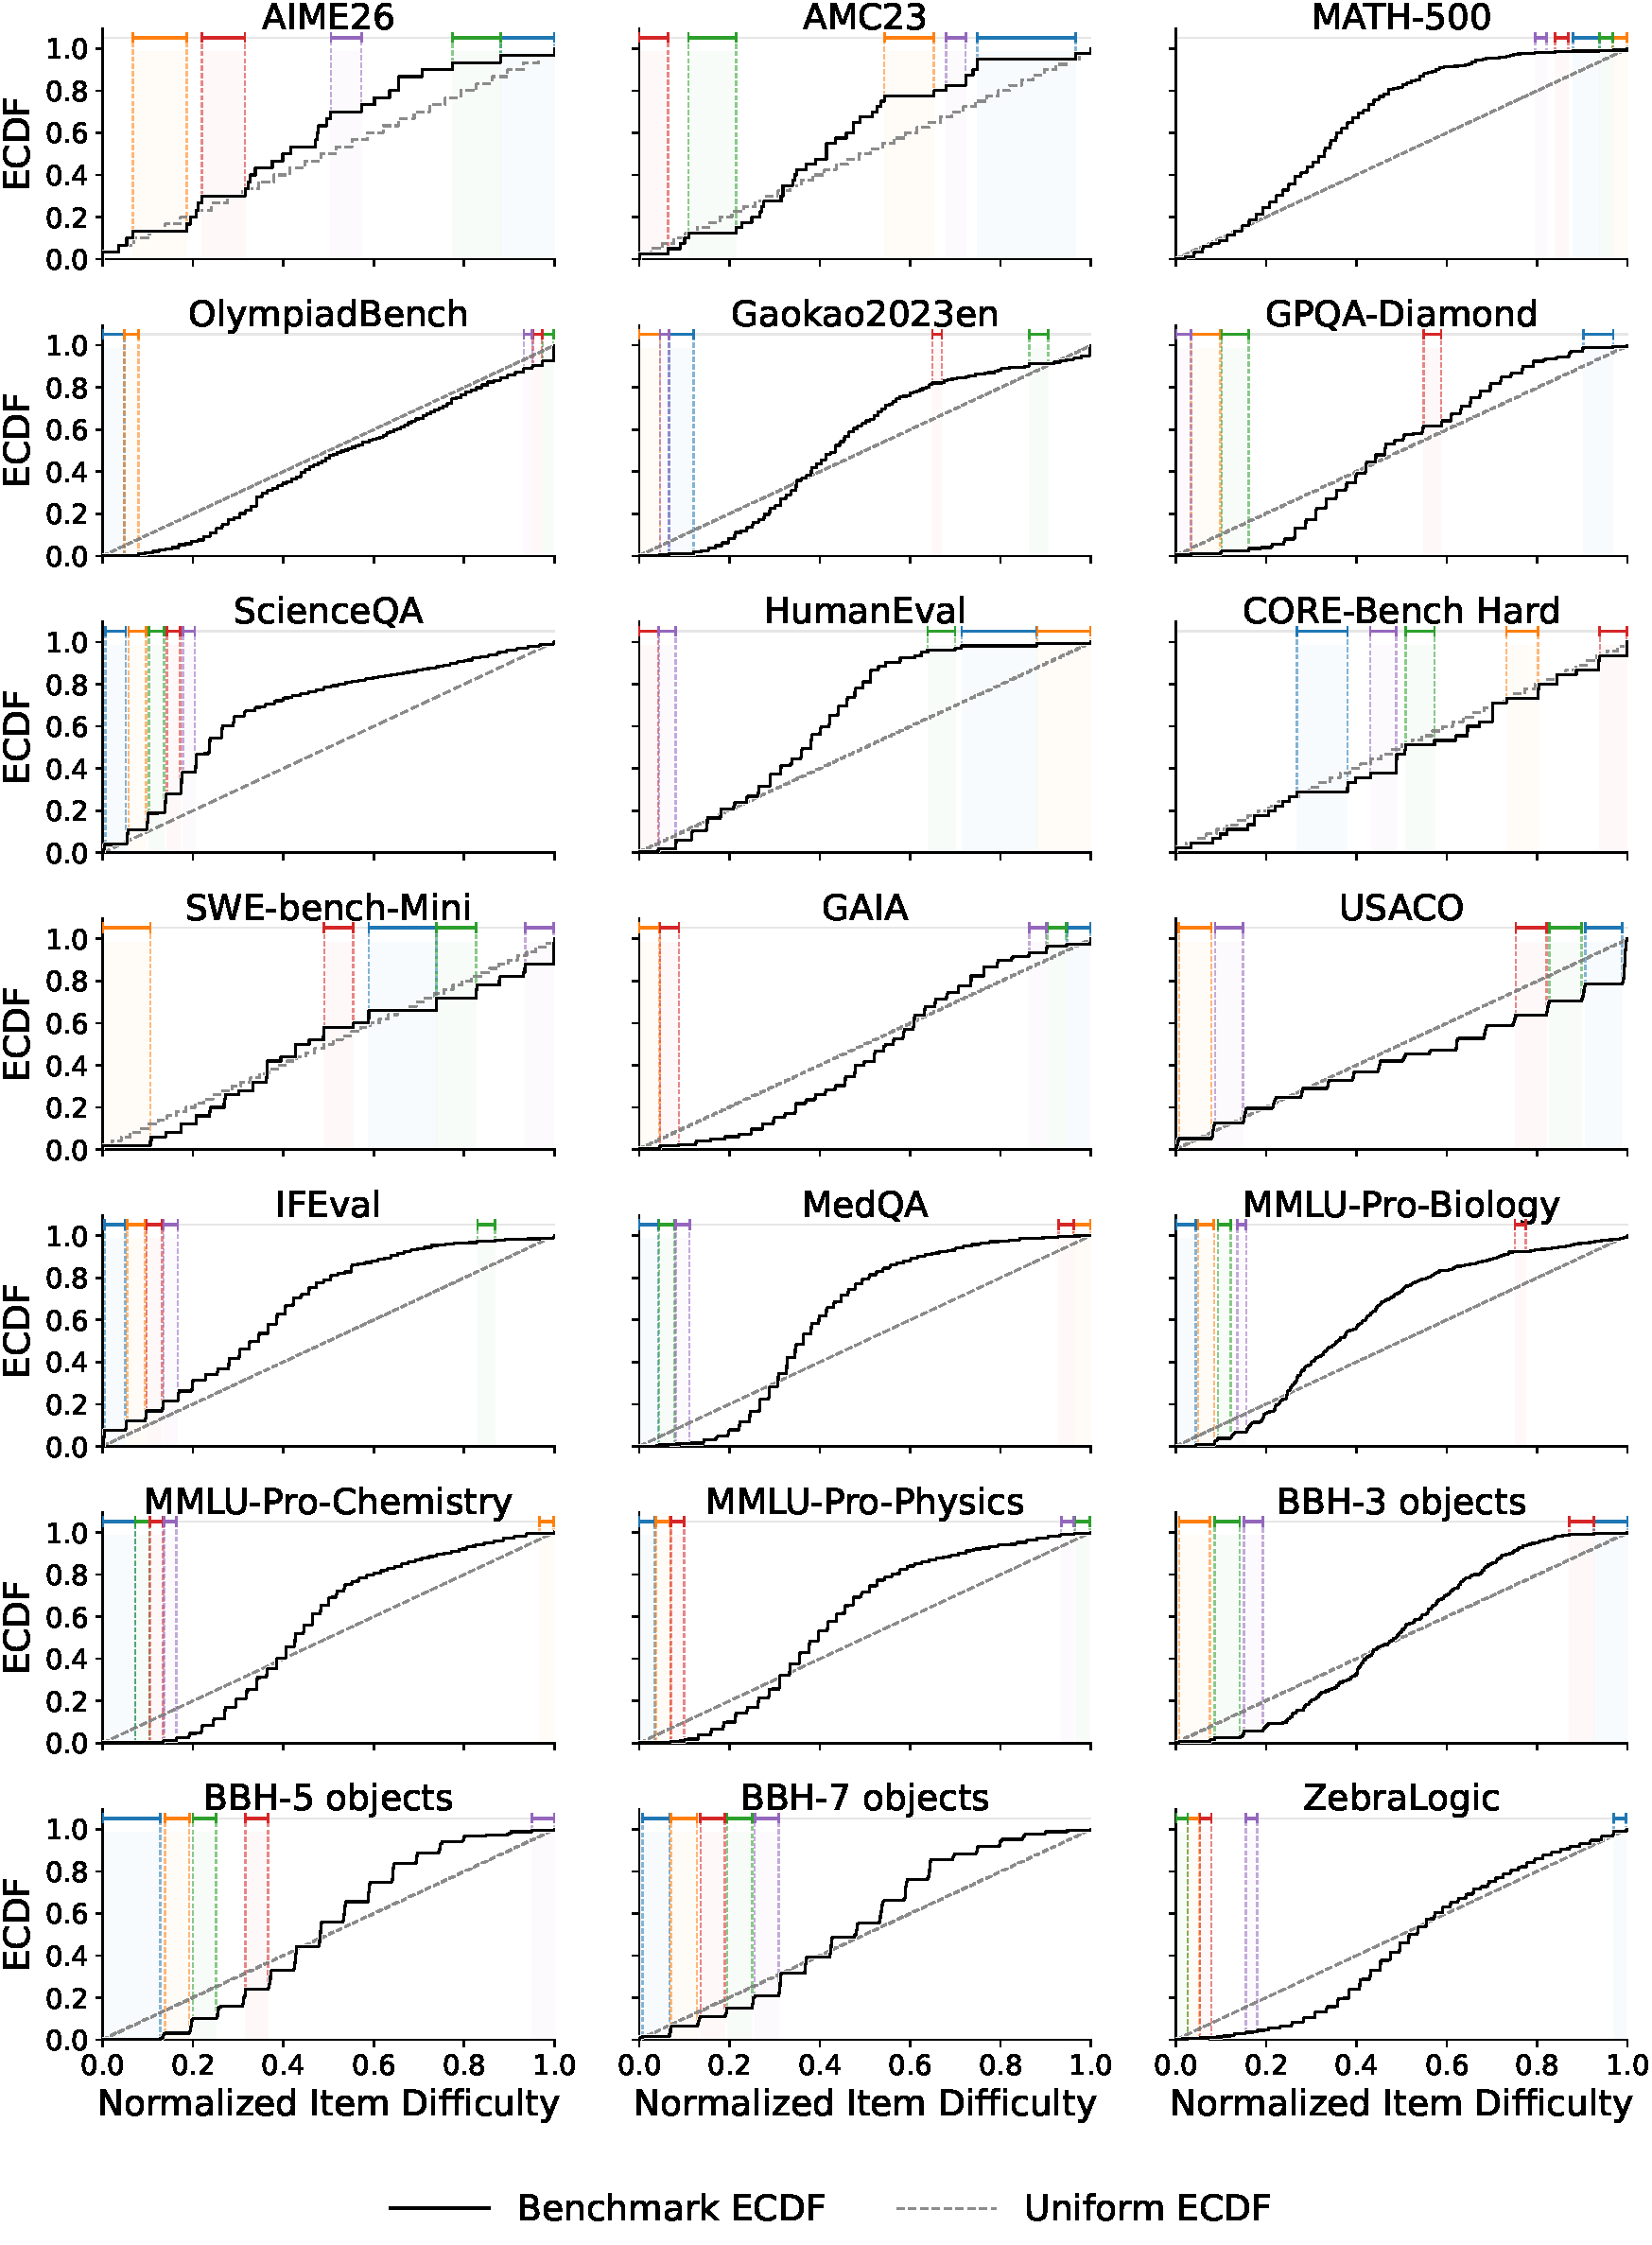
\includegraphics[width=0.95\textwidth,height=0.8\textheight]{Fig/appendix_result.pdf}
    \caption{\textbf{补充的基准难度分布。}
    每个面板展示一个基准归一化题目难度的 ECDF。黑色曲线表示基准 ECDF，灰色虚线表示均匀 ECDF，我们将其用作目标难度分布。偏离均匀 ECDF 表示相对于这一中性目标分布的失配。彩色阴影区间标出排序后题目难度之间五个最大的相邻间隔。}
    \label{fig:appendix_result}
\end{figure*}

\section{基准校准}
\label{sec:app_benchmark_cal}
\paragraph{问题设定。}
测度失配的视角提示了一种重新设计基准的自然方式：调整基准经验测度，使其更好地匹配目标评测分布。考虑基准
\[
B=\{x_1,\ldots,x_n\},
\]
其中每道题 \(x_i\) 具有估计难度 \(z_i\in[0,1]\)。该基准在难度轴上诱导经验测度
\[
\nu_B=\frac{1}{n}\sum_{i=1}^n \delta_{z_i}
\]
。给定目标分布 \(\mu\in\mathcal P([0,1])\)，基准校准旨在构造一个新基准 \(B'\)，使其经验测度 \(\nu_{B'}\) 比 \(\nu_B\) 更接近 \(\mu\)。

在本工作中，我们通过剪枝来实现基准校准。具体而言，我们从原始基准中保留 \(k\) 道题，即选择子集 \(A\subseteq[n]\) 且 \(|A|=k\)。所选题目构成校准后的基准
\[
B_A=\{x_i:i\in A\},
\]
其经验难度测度为
\[
\nu_A=\frac{1}{k}\sum_{i\in A}\delta_{z_i}.
\]
目标是选择 \(A\)，使 \(\nu_A\) 更好地近似目标分布 \(\mu\)，例如以 \(\mathrm{DDM}(B_A;\mu)=W_1(\nu_A,\mu)\) 来衡量。 
% This directly follows the measure-mismatch view: benchmark-induced comparisons are more reliable when the benchmark measure is closer to the intended target measure.

\paragraph{一个简单的校准算法。}
我们使用一个简单的贪心分位数匹配剪枝过程，概括于算法~\ref{alg:benchmark-calibration}。令 \(Q_\mu\) 表示目标分布 \(\mu\) 的分位函数。给定子集大小 \(k\)，我们首先取 \(\mu\) 下 \(k\) 个等概率区间的中点，构造 \(k\) 个目标难度位置：
\[
\tau_t=\frac{t-\frac12}{k},\qquad
q_t=Q_\mu(\tau_t),\qquad t=1,\ldots,k .
\]
然后将这些目标位置匹配到已有基准题。具体而言，在将题目难度归一化到 \([0,1]\) 之后，我们遍历 \(q_1,\ldots,q_k\)，并选择难度最接近当前目标位置的未使用题目：
\[
i_t\in
\arg\min_{i\in [n]\setminus \{i_1,\ldots,i_{t-1}\}}
|z_i-q_t|.
\]
校准子集为 \(A=\{i_1,\ldots,i_k\}\)。

\begin{algorithm}[t]
\caption{分位数匹配的基准校准}
\label{alg:benchmark-calibration}
\begin{algorithmic}[1]
\Require 归一化题目难度 \(z_1,\ldots,z_n\in[0,1]\)，子集大小 \(k\)，目标分位函数 \(Q_\mu\)
\State 初始化已选集合 \(A\leftarrow\emptyset\) 与可用集合 \(U\leftarrow[n]\)
\For{\(t=1,\ldots,k\)}
    \State 设定目标分位水平
    \[
    \tau_t \leftarrow \frac{t-\frac12}{k}
    \]
    \State 设定目标难度位置
    \[
    q_t \leftarrow Q_\mu(\tau_t)
    \]
    \State 选择最接近的未使用题目：
    \[
    i_t \in \arg\min_{i\in U}|z_i-q_t|
    \]
    \State 更新 \(A\leftarrow A\cup\{i_t\}\)
    \State 更新 \(U\leftarrow U\setminus\{i_t\}\)
\EndFor
\State \Return \(A\)
\end{algorithmic}
\end{algorithm}

\subsection{实验设置}

实践中，给定难度轴上的任意目标分布，我们的基准校准想法与算法~\ref{alg:benchmark-calibration} 都可以直接应用。在本实验中，我们研究这种校准能否使单个基准产生的模型排名，与更广泛的同领域基准族更加一致。

我们考虑 \(N=8\) 个数学基准，如表~\ref{tab:benchmark_summary} 所示。对每个基准 \(B_i\)，我们将其视为待校准的源基准，并仅用其余基准 \(\{B_j:j\neq i\}\) 构造模型的外部参照排名。这一留一设计评估：\(B_i\) 的校准版本所诱导的排名，是否与同领域其他基准得到的排名更一致。

具体地，令
\[
B_i=\{x_{i1},\ldots,x_{in_i}\}
\]
为第 \(i\) 个基准，其中题目 \(x_{i\ell}\) 的归一化难度为 \(z_{i\ell}\in[0,1]\)。由于留一参照排名由同领域多个基准汇总而来，它较少受任一源基准特有的难度集中所束缚。因此我们用校准从源基准过度集中的难度区域剪除题目。在没有应用特定目标分布时，我们将校准目标取为均匀分布
\[
\lambda=\mathrm{Unif}[0,1].
\]
这一选择不应被理解为假定留一参照分布恰好是均匀的。相反，均匀校准提供了一种中性的去偏策略：它并不先验地偏袒任何难度区域，并且抵消那些经验质量集中在难度轴狭窄部分的基准。

我们将算法~\ref{alg:benchmark-calibration} 以目标分布 \(\lambda\) 应用于 \(B_i\)，得到大小为 \(k_i\) 的校准子集 \(A_i\subseteq[n_i]\)。校准后的基准为
\[
B_{i,A_i}=\{x_{i\ell}:\ell\in A_i\}.
\]

假设所有基准评估相同的 \(M\) 个模型。令 \(S_i(m)\) 表示模型 \(m\) 在完整源基准 \(B_i\) 上的平均分数，令 \(S_i(A_i,m)\) 表示其在校准子集上的平均分数。未校准排名由
\[
S_i(m),\qquad m=1,\ldots,M,
\]
诱导，而校准排名由
\[
S_i(A_i,m),\qquad m=1,\ldots,M.
\]

对留一参照排名，我们在其余基准上汇总模型分数：
\[
S^{\mathrm{ref}}_{-i}(m)
=
\frac{1}{N-1}\sum_{j\neq i} S_j(m).
\]
由 \(S^{\mathrm{ref}}_{-i}(m)\) 诱导的排名作为源基准 \(B_i\) 的外部参照排名。

对每个源基准，我们计算源诱导排名与留一参照排名之间的 Spearman 与 Kendall 相关，包括校准前与校准后。校准后相关提高，表明把源基准剪枝到更均衡的难度分布，使其模型比较与更广泛的同领域基准族更加一致。

\begin{table*}[t]
\centering
\small
\caption{
\textbf{八个数学基准上的基准校准结果。}
对每个源基准，\textbf{完整}表示原始基准，
\textbf{随机}表示同等规模的 30 个随机剪枝子集的平均，
\textbf{校准}表示我们的分位数匹配基准校准算法产生的校准子集。
Spearman 与 Kendall 衡量与留一参照排名的一致性。
我们报告 \(W_1(\nu,\mathrm{Unif})\) 作为机制指标，以验证校准使所选基准测度更接近中性均匀分布。加粗值表示每个基准、每个指标上 \textbf{完整}、\textbf{随机} 与 \textbf{校准} 中的最佳结果。
}
\label{tab:benchmark_calibration}
\begin{adjustbox}{width=\textwidth}
\begin{tabular}{lccccccccc}
\toprule
& \multicolumn{3}{c}{\textbf{Spearman $\uparrow$}}
& \multicolumn{3}{c}{\textbf{Kendall $\uparrow$}}
& \multicolumn{3}{c}{\(\boldsymbol{W_1(\nu,\mathrm{Unif})}\) \(\boldsymbol{\downarrow}\)} \\
\cmidrule(lr){2-4}
\cmidrule(lr){5-7}
\cmidrule(lr){8-10}
\textbf{基准}
& \textbf{完整} & \textbf{随机} & \textbf{校准}
& \textbf{完整} & \textbf{随机} & \textbf{校准}
& \textbf{完整} & \textbf{随机} & \textbf{校准} \\
\midrule
Minerva-Math  & 0.601 & 0.649 & \textbf{0.790} & 0.455 & 0.514 & \textbf{0.667} & 0.122 & 0.115 & \textbf{0.005} \\
MATH-500      & 0.930 & 0.942 & \textbf{0.958} & 0.879 & 0.878 & \textbf{0.909} & 0.164 & 0.165 & \textbf{0.099} \\
Gaokao2023en  & 0.888 & 0.895 & \textbf{0.951} & 0.788 & 0.790 & \textbf{0.879} & 0.088 & 0.086 & \textbf{0.029} \\
AIME24        & \textbf{0.944} & 0.942 & \textbf{0.944} & \textbf{0.848} & 0.847 & \textbf{0.848} & 0.077 & 0.108 & \textbf{0.019} \\
AIME25        & 0.958 & 0.936 & \textbf{0.972} & 0.909 & 0.854 & \textbf{0.915} & 0.079 & 0.126 & \textbf{0.020} \\
AIME26        & 0.949 & 0.950 & \textbf{0.970} & 0.870 & 0.867 & \textbf{0.901} & 0.085 & 0.108 & \textbf{0.017} \\
AMC23         & \textbf{0.937} & 0.934 & \textbf{0.937} & \textbf{0.848} & \textbf{0.848} & \textbf{0.848} & 0.089 & 0.093 & \textbf{0.025} \\
OlympiadBench & \textbf{0.916} & 0.910 & \textbf{0.916} & \textbf{0.818} & 0.806 & \textbf{0.818} & 0.064 & 0.067 & \textbf{0.008} \\
\midrule
平均       & 0.890 & 0.895 & \textbf{0.930} & 0.802 & 0.801 & \textbf{0.848} & 0.096 & 0.109 & \textbf{0.028} \\
\bottomrule
\end{tabular}
\end{adjustbox}
\end{table*}
\subsection{结果}

实验结果见表~\ref{tab:benchmark_calibration}。结果表明，我们的校准算法提高了源基准排名与留一参照排名之间的一致性。平均而言，校准将 Spearman 相关从 \(0.890\) 提高到 \(0.930\)，将 Kendall 相关从 \(0.802\) 提高到 \(0.848\)。改进在初始一致性较弱的基准上尤其明显。值得注意的是，在 Minerva-Math 上，完整基准与参照排名的 Spearman 与 Kendall 相关分别只有 \(0.601\) 与 \(0.455\)，而校准将其分别提高到 \(0.790\) 与 \(0.667\)。类似地，在 Gaokao2023en 上，校准将 Spearman 从 \(0.888\) 提高到 \(0.951\)，将 Kendall 从 \(0.788\) 提高到 \(0.879\)。对其余基准，初始一致性已经很高，改进空间较小；尽管如此，校准在使用剪枝后基准的同时，始终保持了这一高水平一致性。

我们加入一个随机剪枝基线，其剪枝规模与校准子集相同，并在 30 次随机试验上取平均。随机剪枝不如校准有效：它的平均 Spearman 为 \(0.895\)，平均 Kendall 为 \(0.801\)，都低于校准子集。我们还报告 \(W_1(\nu,\mathrm{Unif})\) 作为机制指标。校准在所有基准上一致地减小该距离，将平均值从 \(0.096\) 降到 \(0.028\)。相反，随机剪枝平均而言并不减小该距离，平均值为 \(0.109\)。这表明改进并非仅仅因为使用了更小的基准，而是来自选择那些经验难度测度更好地匹配中性校准目标的题目。


\section{\textsc{BenchFill} 的补充细节与实验结果}



\newpage
\begin{algorithm}[t]
\caption{\textsc{BenchFill}}
\label{alg:gap_filling}
\begin{algorithmic}[1]
\Require 带归一化难度的基准题 $\{(x_i,z_i)\}_{i=1}^n$；目标间隔 $[z_L,z_R]$；改写 LLM $\mathcal{G}$；有效性评判器 $\mathcal{J}$；IRT 评测 LLM $\{M_j\}_{j=1}^m$ 及其预先估计的 IRT 能力 $\{\hat{\theta}_j\}_{j=1}^m$；每个 LLM 的试验次数 $\{K_j\}_{j=1}^m$；父题数 $R$；每个父题的子题数 $C$；参照列表预算 $L$；最大轮数 $T$；归一化 $[0,1]$ 标尺上的容差 $\tau$。
\Ensure 一道提议的缺口填补题目 $x^\star_{\mathrm{item}}$。

\State 设定目标难度 $z^\star \gets (z_L+z_R)/2$。
\State 用所选间隔附近已有的标注题目--难度对初始化记忆 $\mathcal{M}$。
\State 初始化有效候选集 $\mathcal{C}_{\mathrm{valid}} \gets \emptyset$。

\For{$t=1,\dots,T$}
    \State 检索父题集 $\mathcal{S}_t \subseteq \mathcal{M}$，其中至多 $R$ 道题，其标注难度最接近 $z^\star$。
    \State 用 $z^\star$ 附近的题目--难度对构造参照列表 $\mathcal{R}_t \subseteq \mathcal{M}$，满足 $|\mathcal{R}_t|\le L$；在可得时，至多一半取自低于 $z^\star$ 的题目，其余取自高于 $z^\star$ 的题目。
    
    \For{每个父题 $(x_p,z_p) \in \mathcal{S}_t$}
        \State 为了提示，将 $z^\star$ 与 $\mathcal{R}_t$ 中显示的难度从 $[0,1]$ 重新缩放到 $[0,10]$。
        \State 以父题、目标难度和参照列表为条件，将父题改写为 $C$ 个子题：
        \[
        \{x_{p,1},\dots,x_{p,C}\}
        \gets
        \mathcal{G}(x_p, z^\star, \mathcal{R}_t).
        \]
        
        \For{每个子题 $x_{p,c}$}
            \If{$\mathcal{J}$ 核验 $x_{p,c}$ 的参考答案正确}
                \For{$j=1,\dots,m$}
                    \State 用 LLM $M_j$ 在 $x_{p,c}$ 上做 $K_j$ 次试验，并记录 $c_j$ 次正确回答。
                \EndFor
                \State 通过在线校准估计题目难度：
                \[
                \hat{b}_{p,c}
                \gets
                \arg\max_b
                \sum_{j=1}^{m}
                \left[
                c_j\log \sigma(\hat{\theta}_j-b)
                +
                (K_j-c_j)\log\bigl(1-\sigma(\hat{\theta}_j-b)\bigr)
                \right].
                \]
                \State 用与原始基准相同的变换归一化 $\hat{b}_{p,c}$，得到 $\hat{z}_{p,c}$。
                \State 将 $(x_{p,c},\hat{z}_{p,c})$ 加入 $\mathcal{M}$。
                \State 将 $(x_{p,c},\hat{z}_{p,c})$ 加入 $\mathcal{C}_{\mathrm{valid}}$。
            \EndIf
        \EndFor
    \EndFor
    
    \If{$\mathcal{C}_{\mathrm{valid}} \neq \emptyset$ and
    $\min_{(x,\hat{z})\in \mathcal{C}_{\mathrm{valid}}} |\hat{z}-z^\star| \le \tau$}
        \State \textbf{跳出}
    \EndIf
\EndFor

\If{$\mathcal{C}_{\mathrm{valid}} = \emptyset$}
    \State \Return 失败
\EndIf

\State 选择最接近的有效子题：
\[
(x^\star_{\mathrm{item}},\hat{z}^\star)
\gets
\arg\min_{(x,\hat{z})\in \mathcal{C}_{\mathrm{valid}}}
|\hat{z}-z^\star|.
\]
\State \Return $x^\star_{\mathrm{item}}$ 作为提议的缺口填补题目，并交由人类专家审核。
\end{algorithmic}
\end{algorithm}

\subsection{实现细节}
\label{sec:app_gap}


对每个基准，我们关注其估计难度分布中三个最显著的间隔，并为每个间隔改写一道题。由于当提示中给出目标难度时，LLM 可能无法可靠区分归一化 $[0,1]$ 难度标尺上的细小数值差异，我们在提示时将难度值重新缩放到 $[0,10]$，而所有报告的指标仍保持在原始归一化标尺上。

对参照列表，我们在目标难度两侧都纳入附近的题目--难度对。具体而言，一半参照题选自难度低于目标且最接近目标的题目，另一半选自难度高于目标且最接近目标的题目。这为改写器提供了期望难度水平附近的局部双向上下文。完整的改写提示模板如下。

对难度标注，我们使用与原始难度估计阶段相同的 LLM 集合和相同的生成配置。若迄今找到的最佳有效题目在归一化 $[0,1]$ 标尺上与目标难度的距离处于容差 $\tau=0.01$ 之内，搜索提前停止；否则在达到最大轮数后停止。然后我们选择标注难度最接近目标的有效题目。在插入基准之前，每道入选题目都由至少三位人类专家进行人工有效性检查，以核验其正确性。

我们额外实现了一个预算匹配的 best-of-\(N\) 均匀父题改写基线。对每个目标间隔 \(g\)，令 \(T_g\) 表示 \textsc{BenchFill} 在停止前实际运行的轮数。由于 \textsc{BenchFill} 每轮改写 \(4\) 个父题、每个父题产生 \(4\) 个子题，该间隔的提议预算为 \(T_g \times 4 \times 4 = 16T_g\) 个子题。为匹配这一预算，基线均匀抽取 \(4\) 道已有基准题作为父题，并让同一个改写 LLM 以父题和目标难度为条件，从每个父题改写出 \(4T_g\) 个子题。难度标注之后，它在所有生成候选中选择难度最接近目标的有效子题。因此，基线使用与 \textsc{BenchFill} 相同的总改写预算和相同的最终选择规则，但不使用难度感知的父题检索、附近参照列表或迭代记忆更新。

\begin{center}
\begin{tcolorbox}[
    title={改写器提示模板},
    label={box:proposer_prompt},
    width=\linewidth,
    colback=white,
    colframe=black,
    boxrule=0.5pt,
    left=6pt,
    right=6pt,
    top=6pt,
    bottom=6pt,
    fonttitle=\bfseries,
    fontupper=\ttfamily\small,
]

将下面的父题改写为\textbf{恰好 1} 道新的基准题变体。
目标难度（0--10 标尺，越高越难）：
\textbf{\{target\_difficulty\}}。

\medskip
\textbf{父题}（将此题改写为新变体——不要复制其具体措辞、数字或答案）：

\{parent.question\}

答案：\{parent.reference\_answer\}

难度（0--10）：\{parent.difficulty\} $|$ delta \{target - parent.difficulty\} $|$ generate \texttt{\{harder|easier\}}

\medskip
\textbf{记忆题目}（仅用作风格/难度参照，不要复制）：

\medskip
--- 记忆 1 ---

\{memory[0].question\}

答案：\{memory[0].reference\_answer\}

难度（0--10）：\{memory[0].difficulty\} $|$ delta \{target - memory[0].difficulty\} $|$ generate \texttt{\{harder|easier\}}

\medskip
--- 记忆 2 ---

\{memory[1].question\}

答案：\{memory[1].reference\_answer\}

难度（0--10）：\{memory[1].difficulty\} $|$ delta \{target - memory[1].difficulty\} $|$ generate \texttt{\{harder|easier\}}

\medskip
...（每个记忆题目一块）...

\medskip
\textbf{只}返回一个 markdown 代码块：第一行以 \texttt{\textasciigrave\textasciigrave\textasciigrave{}json} 开始，然后换行，然后是一个\textbf{恰好含 1} 个元素的 JSON 数组，再单独一行以 \texttt{\textasciigrave\textasciigrave\textasciigrave} 结束。结束围栏之后不要放任何内容。

\medskip
在 JSON \textbf{语法完整}之前不要停止：每个字符串值都以 \texttt{"} 闭合，每个对象都以 \texttt{\}} 闭合，数组以 \texttt{]} 结束，然后是结束用的 \texttt{\textasciigrave\textasciigrave\textasciigrave} 行。

\medskip
该数组必须\textbf{恰好含 1} 个元素——一个对象，且恰好包含这些键：
\texttt{"id"}（字符串），\texttt{"question"}（字符串），\texttt{"answer"}（字符串）。

\end{tcolorbox}
\end{center}

\subsection{补充实验结果}

% \naicheng{human validation; Does the rewriter perceive difficulty?}

% \jiawen{Empirical Validation beyond gap reduction}

\paragraph{人工验证。}
我们用两阶段验证过程确保生成的缺口填补题目可靠。GPT-5.4 首先作为自动有效性评判器，检查每个候选是否格式良好、其参考答案是否正确；未通过该检查的候选被丢弃并重新生成。人类专家随后独立审核最终入选的题目。在 24 个目标间隔中，有一个最初提议的候选因参考答案错误而未通过 GPT-5.4 检查，并被重新生成。全部 24 道最终入选题目都通过了 GPT-5.4 有效性检查，并随后未经修改或替换地通过了人工审核。

\paragraph{改写器能否感知难度？} 一个自然的问题是，我们的改写器是否确实感知难度，而不是盲目地命中目标难度。我们从两个互补角度考察这一问题：改写器在迭代反馈之前是否已经表现出难度敏感性，以及随后的搜索并标注循环是否进一步提高与目标难度的对齐。

首先，为了把改写器自身的难度感知与后来的 IRT 反馈及迭代搜索隔离开，我们只分析每个缺口填补情形的第一轮生成。在此阶段，改写器以指定的目标难度为条件，但尚未收到其生成子题的标注难度反馈。图~\ref{fig:first_round_calibration} 展示了全部 8 个基准、每个基准 3 个目标间隔上，指定目标难度与有效首轮子题的标注难度。在大多数基准内，更高的指定目标产生更高的平均标注难度，并且分隔良好的目标通常诱导出不同的子题难度分布。这表明，在引入迭代反馈之前，改写器对指定难度标尺已经具有非平凡的敏感性。

其次，我们考察搜索并标注循环是否进一步提高目标对齐。图~\ref{fig:multi_round_deviation} 展示了每个基准中一个有代表性的缺口填补情形。在这些情形中，平均绝对目标偏差总体上从第一轮下降到最后一轮，并且在大多数情形中生成的子题也更集中于目标附近。这表明，迭代循环利用 IRT 标注与更新后的记忆，进一步细化了改写器最初的难度信号。

\begin{figure*}[t]
    \centering
    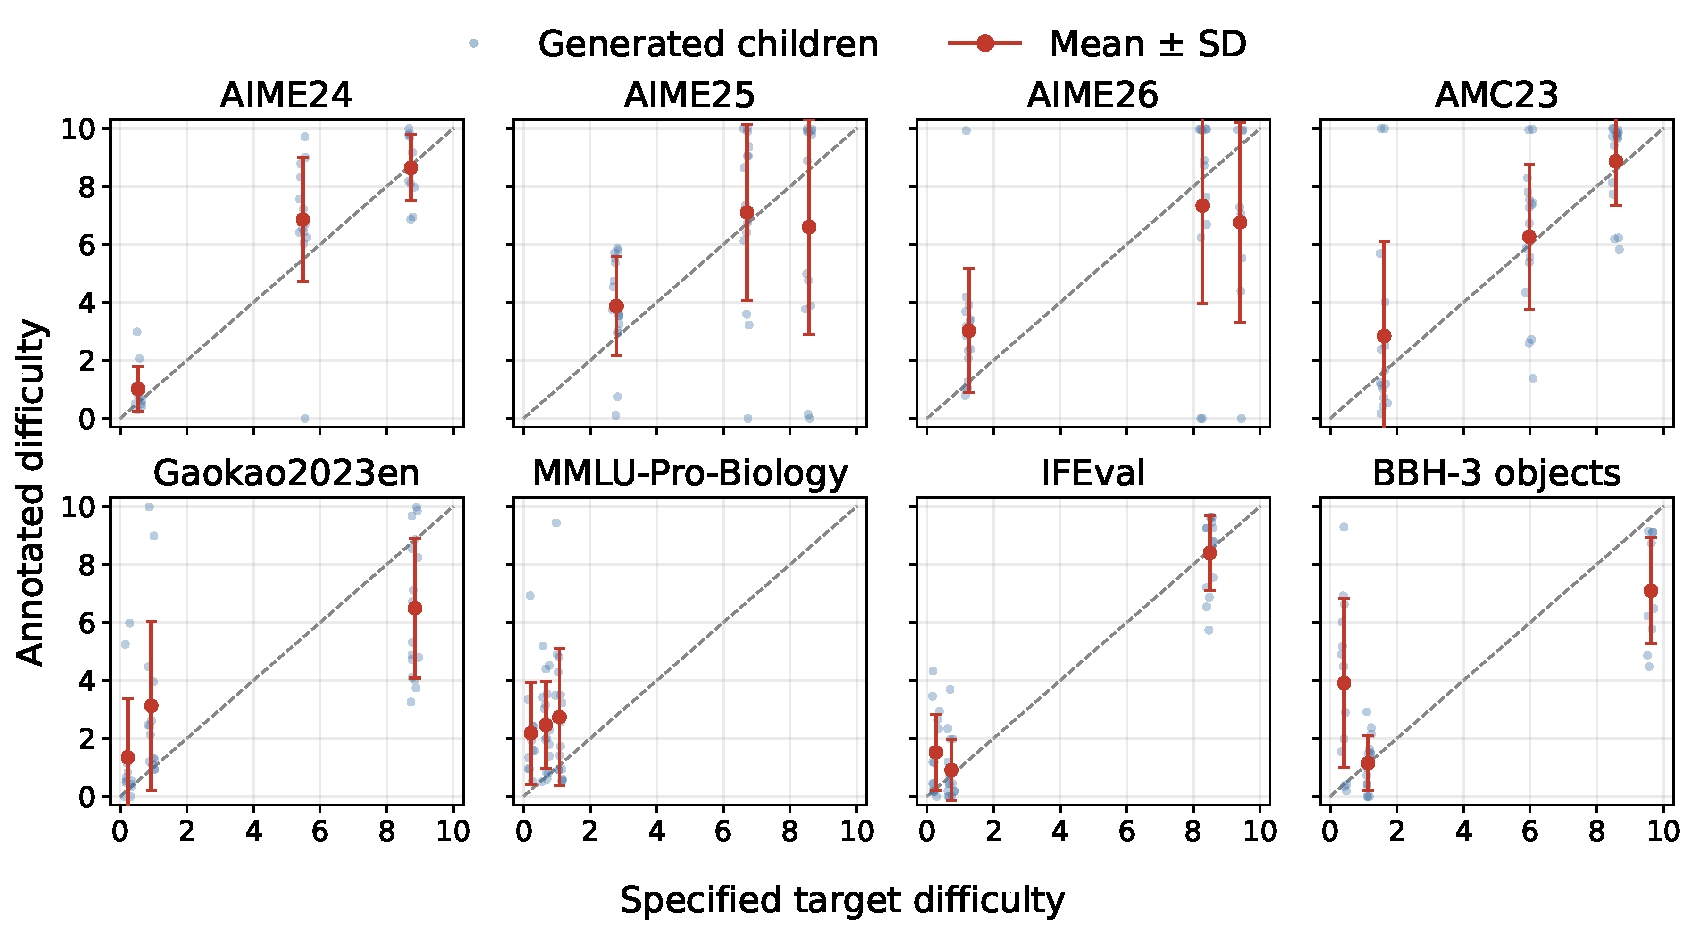
\includegraphics[width=\textwidth]{Fig/first_round_calibration.pdf}
    \caption{\textbf{指定目标难度与标注难度的首轮对齐。}
    每个面板对应一个基准。横轴为指定目标难度，纵轴为有效首轮子题的标注难度。蓝点表示单个生成子题，红色标记表示每个目标难度的均值与标准差。虚线对角线表示完全对齐。为便于阅读，两个坐标轴都显示在 0--10 标尺上，对应于 $[0,1]$ 中的归一化难度乘以 10。在大多数基准内，更高的指定目标在第一轮、即纳入任何迭代反馈之前，就已经产生更高的标注难度。}
    \label{fig:first_round_calibration}
\end{figure*}


\begin{figure*}[t]
    \centering
    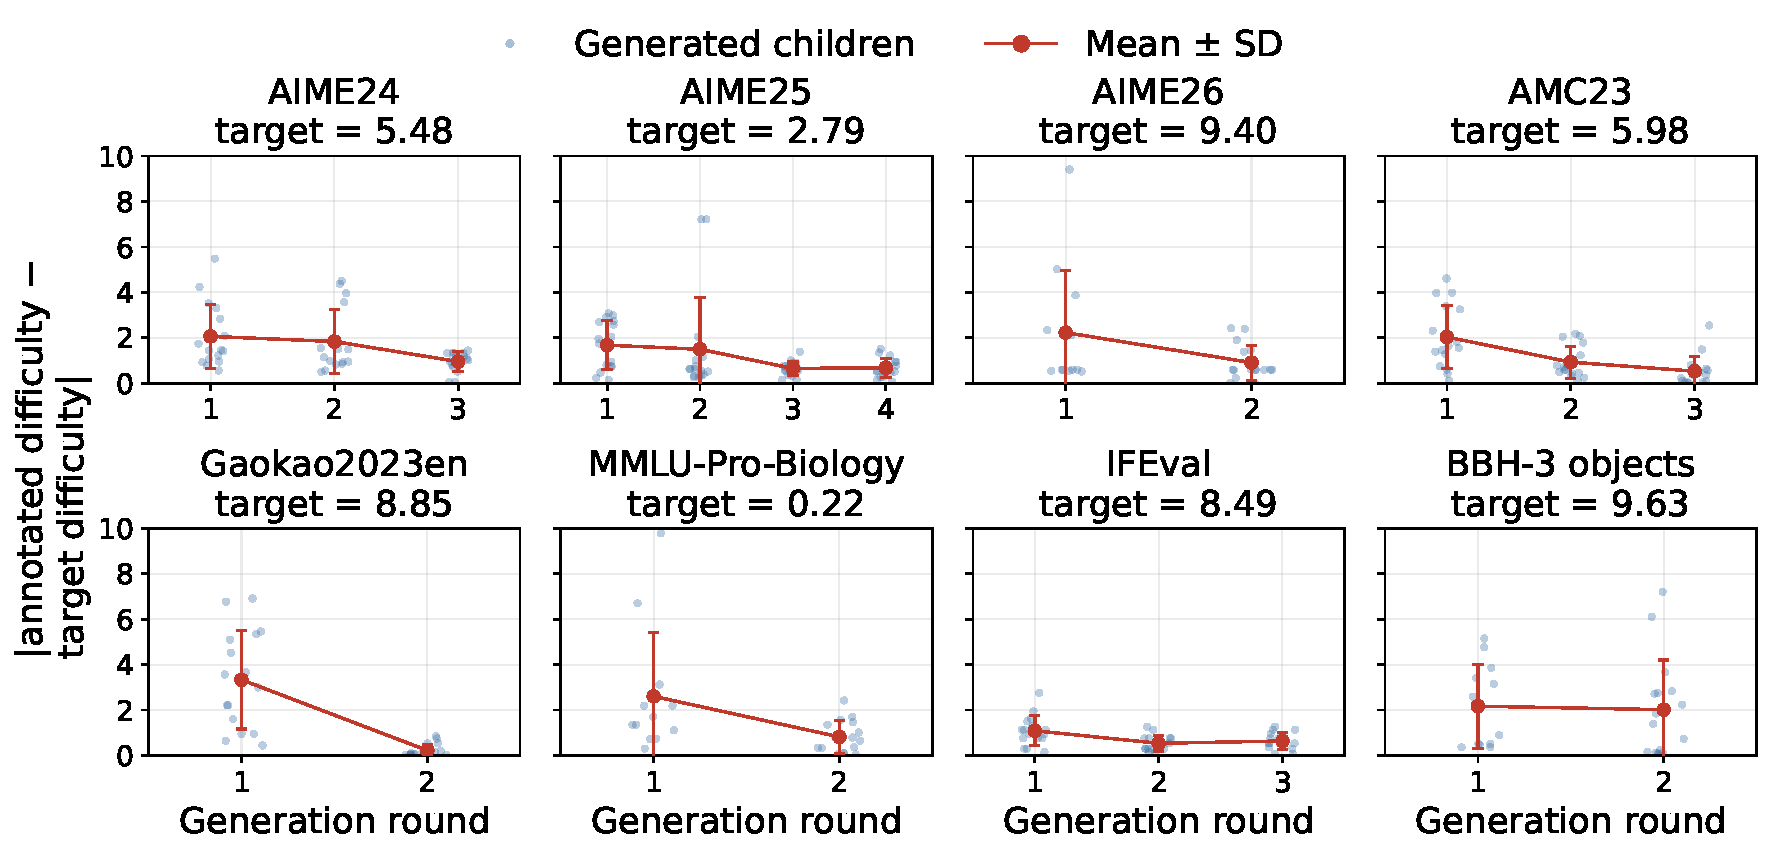
\includegraphics[width=\textwidth]{Fig/multiround_target_deviation.pdf}
    \caption{\textbf{\textsc{BenchFill} 搜索过程中的多轮目标对齐。}
    每个面板展示来自不同基准的一个有代表性的缺口填补情形。横轴为生成轮次，纵轴为生成子题的绝对目标偏差 $|\hat{z} - z^\star|$。为便于阅读，目标难度与绝对偏差都乘以 10。蓝点表示单个生成子题，红色标记表示该轮的均值与标准差。
    在大多数情形中，平均目标偏差随轮次下降，生成的子题更集中于目标附近，表明搜索并标注循环在改写器最初的难度敏感性之外进一步提高了目标对齐。}
    \label{fig:multi_round_deviation}
\end{figure*}


\paragraph{检测局部模型改进。}
我们进一步考察 \textsc{BenchFill} 是否在缩小难度间隔之外，提高基准检测局部模型改进的能力。我们在 AIME24、AIME25 与 AIME26 中各考虑一个目标间隔，并比较三种基准变体：\texttt{原始}、\texttt{原始 + BenchFill} 与 \texttt{原始 + 基线}。两种扩充方法都向原始基准恰好插入一道题。我们进行轻度 SFT，使模型在目标间隔区域附近得到改进。每道题在 SFT 前后各用 32 次 rollout 评估，并用单侧分层随机化检验（$p<0.05$）检验增益是否在统计上可检测。

如表~\ref{tab:localized_detection} 所示，\texttt{原始 + BenchFill} 在全部三个情形中都检测到 SFT 后的正增益（3/3），而 \texttt{原始} 与 \texttt{原始 + 基线} 都没有检测到（各为 0/3）。这表明 \textsc{BenchFill} 并非仅仅改进它所优化的指标；通过填补覆盖不足的难度区域，它使基准对否则会被遗漏的局部模型改进更加敏感。



\begin{table*}[t]
\centering
\caption{\textbf{局部改进检测结果。}
每种扩充方法都向原始的 30 题基准增加一道题。
增益表示平均准确率的变化。
单侧分层随机化检验在每道题内，用 100{,}000 次置换将 rollout 结果在 SFT 前与 SFT 后条件之间随机重新分配。
加粗表示在 $p<0.05$ 下检测到正增益的变体。}
\label{tab:localized_detection}
\small
\setlength{\tabcolsep}{5pt}
\begin{tabular}{llccc}
\toprule
\textbf{情形}
& \textbf{基准变体}
& \textbf{增益}
& \textbf{单侧 $p$}
& \textbf{是否检出} \\
\midrule
\multirow{3}{*}{\shortstack[l]{AIME24\\Olmo-3.1-32B-Think}}
& \texttt{原始}
& +0.104 & 0.500100 & $\times$ \\
& \textbf{\texttt{原始 + BenchFill}}
& \textbf{+2.419} & \textbf{0.005940} & $\checkmark$ \\
& \texttt{原始 + 基线}
& +0.202 & 0.458000 & $\times$ \\
\midrule
\multirow{3}{*}{\shortstack[l]{AIME25\\Phi-4}}
& \texttt{原始}
& +1.042 & 0.184100 & $\times$ \\
& \textbf{\texttt{原始 + BenchFill}}
& \textbf{+3.730} & \textbf{0.000450} & $\checkmark$ \\
& \texttt{原始 + 基线}
& +0.907 & 0.214200 & $\times$ \\
\midrule
\multirow{3}{*}{\shortstack[l]{AIME26\\Llama-3.1-8B-Instruct}}
& \texttt{原始}
& +0.208 & 0.418400 & $\times$ \\
& \textbf{\texttt{原始 + BenchFill}}
& \textbf{+3.427} & \textbf{0.000010} & $\checkmark$ \\
& \texttt{原始 + 基线}
& +0.101 & 0.498000 & $\times$ \\
\bottomrule
\end{tabular}
\end{table*}

\paragraph{代表性示例。}
为定性展示生成的缺口填补题目，我们在表~\ref{tab:gap_filling_examples} 中给出有代表性的改写示例。每个示例同时给出最终入选题目及其在基准中的原始祖先，以及祖先难度、目标难度和入选题目的标注难度。这些示例说明 \textsc{BenchFill} 如何修改已有基准题，以到达先前覆盖不足的难度水平。



% To illustrate how \textsc{BenchFill} approaches the target difficulty over multiple rounds, we provide several example search trajectories in Fig.~\ref{fig:gap_filling_examples}. Each subplot corresponds to one benchmark--gap pair. These examples provide a qualitative view of how the rewrite-and-annotate search progressively moves toward the target difficulty. We also provide representative rewriting examples in Tab.~\ref{tab:gap_filling_examples}, showing each final selected item together with its original ancestor item from the benchmark, as well as the target difficulty and annotated difficulty of the selected item.


% \begin{figure*}[t]
%     \centering
%     \includegraphics[width=\textwidth]{Fig/gap_example.pdf}
%     \caption{\textbf{Example \textsc{BenchFill} search trajectories.}
%     Each panel shows one gap-filling example for a specific benchmark--gap pair.
%     The horizontal axis denotes the search round, and the vertical axis denotes the absolute deviation between the best valid item found up to round $t$ and the target difficulty,
%     $\left|\hat{z}_{\mathrm{best}}^{(t)} - z^\star\right|$.
%     Values closer to zero indicate better alignment with the target difficulty.
%     The tolerance band is set to $0.01$, and the search terminates once the best valid item falls within this band.
%     The decreasing trajectories show that \textsc{BenchFill} progressively finds valid items closer to the target difficulty.}
%     \label{fig:gap_filling_examples}
% \end{figure*}

% \begin{table*}[t]
% \centering
% \footnotesize
% \setlength{\tabcolsep}{2.5pt}
% \renewcommand{\arraystretch}{1.15}
% \caption{
% \textbf{Representative pairs of original benchmark ancestors and final selected items produced by \textsc{BenchFill}.}
% All difficulty values are normalized to $[0,1]$.
% The main change from the ancestor item to the selected item is highlighted. For selected items, values in parentheses denote the target difficulty.
% }
% \label{tab:gap_filling_examples}
% \begin{tabularx}{\textwidth}{
% >{\centering\arraybackslash}p{0.125\textwidth}
% >{\hspace{3pt}\raggedright\arraybackslash}p{0.275\textwidth}
% >{\centering\arraybackslash}p{0.070\textwidth}
% >{\raggedright\arraybackslash}p{0.395\textwidth}
% >{\centering\arraybackslash}p{0.090\textwidth}
% }
% \toprule
% \textbf{Benchmark}
% & \multicolumn{2}{c}{\textbf{Original benchmark ancestor}}
% & \multicolumn{2}{c}{\textbf{Selected gap-filling item}} \\
% \cmidrule(lr){2-3}
% \cmidrule(lr){4-5}
% & \multicolumn{1}{c}{\textbf{Item}}
% & \textbf{Diff.}
% & \multicolumn{1}{c}{\textbf{Item}}
% & \shortstack{\textbf{Diff.}} \\
% \midrule

% \textbf{AMC23}
% &
% For how many ordered pairs $(a,b)$ of integers does the polynomial $x^3+ax^2+bx+\colorbox{red!20}{6}$ have $3$ distinct integer roots?
% &
% $0.749$
% &
% Find the number of ordered pairs $(a,b)$ of integers such that the polynomial $x^3+ax^2+bx+\colorbox{red!20}{60}$ has exactly three distinct integer roots.
% &
% $0.859$ $(0.857)$
% \\

% \midrule

% \textbf{Gaokao2023en}
% & On an \colorbox{red!20}{$8 \times 8$ chessboard,} \colorbox{red!20}{6 black rooks} and $k$ white rooks are placed on different cells so that each rook only attacks rooks of the opposite color. Compute the maximum possible value of $k$. Two rooks attack each other if they are in the same row or column and no rooks are between them.
% &
% $0.864$
% & On a \colorbox{red!20}{$10 \times 10$ toroidal chessboard}, where the first and last rows are adjacent and the first and last columns are adjacent, \colorbox{red!20}{7 black rooks} and $k$ white rooks are placed on distinct squares such that no rook attacks another rook of the same color. A rook attacks another if they share a row or column with no intervening rooks; on this board, this condition applies in both directions along the row or column. Determine the maximum possible value of $k$.
% &
% $0.882$ $(0.885)$
% \\

% \midrule

% \textbf{AIME25}
% &
% The $27$ cells of a $3 \times 9$ grid are filled with the numbers $1$ through $9$ so that each row contains $9$ different numbers and each $3 \times 3$ block contains $9$ different numbers, as in the first three rows of a Sudoku puzzle. The number of different ways to fill \colorbox{red!20}{such a grid} can be written as $p^a q^b r^c s^d$, where $p,q,r,s$ are distinct primes and $a,b,c,d$ are positive integers. Find $pa+qb+rc+sd$.
% &
% $0.592$
% &
% The $27$ cells of a $3 \times 9$ grid are filled with the numbers $1$ through $9$ so that each row contains $9$ different numbers and each $3 \times 3$ block contains $9$ different numbers, as in the first three rows of a Sudoku puzzle. The number of different ways to fill such a grid \colorbox{red!20}{such that the first column contains the} \colorbox{red!20}{numbers $1,2,3$} in that order can be written as $p^a q^b r^c s^d$, where $p,q,r,s$ are distinct primes and $a,b,c,d$ are positive integers. Find $pa+qb+rc+sd$.
% &
% $0.675$ $(0.671)$
% \\

% \bottomrule
% \end{tabularx}
% \end{table*}

\begin{table*}[t]
\centering
\footnotesize
\setlength{\tabcolsep}{2.5pt}
\renewcommand{\arraystretch}{1.15}
\caption{
\textbf{\textsc{BenchFill} 产生的原始基准祖先与最终入选题目的代表性配对。}
所有难度值都归一化到 $[0,1]$。
从祖先题目到入选题目的主要改动被高亮。对入选题目，括号中的值表示目标难度。
}
\label{tab:gap_filling_examples}
\begin{tabularx}{\textwidth}{
>{\centering\arraybackslash}p{0.125\textwidth}
>{\hspace{3pt}\raggedright\arraybackslash}p{0.275\textwidth}
>{\centering\arraybackslash}p{0.070\textwidth}
>{\raggedright\arraybackslash}p{0.395\textwidth}
>{\centering\arraybackslash}p{0.090\textwidth}
}
\toprule
\textbf{基准}
& \multicolumn{2}{c}{\textbf{原始基准祖先}}
& \multicolumn{2}{c}{\textbf{入选的缺口填补题目}} \\
\cmidrule(lr){2-3}
\cmidrule(lr){4-5}
& \multicolumn{1}{c}{\textbf{题目}}
& \textbf{难度}
& \multicolumn{1}{c}{\textbf{题目}}
& \shortstack{\textbf{难度}} \\
\midrule

\textbf{AMC23}
&
对多少个整数 $n$，表达式 $\sqrt{\frac{\log (n^2) - (\log n)^2}{\log n - \colorbox{red!20}{3}}}$ 表示一个实数，其中 $\log$ 表示以 $10$ 为底的对数？
&
$0.535$
&
求使得 $\sqrt{\frac{\log (n^2) - (\log n)^2}{\log n - \colorbox{red!20}{1}}}$ 表示实数的整数 $n$ 的个数，其中 $\log$ 表示以 $10$ 为底的对数。
&
$0.597$ $(0.598)$
\\

\midrule

\textbf{Gaokao2023en}
& 在一个\colorbox{red!20}{$8 \times 8$ 的棋盘上}放置\colorbox{red!20}{$6$ 枚黑车}和 $k$ 枚白车，且它们位于不同格子，使得每枚车只攻击相反颜色的车。求 $k$ 的最大可能值。（若两枚车位于同一行或同一列且中间没有其他车，则它们互相攻击。）
&
$0.864$
& 在一个\colorbox{red!20}{$9 \times 9$ 的棋盘上}放置\colorbox{red!20}{$7$ 枚黑车}和 $k$ 枚白车，且它们位于不同格子，使得每枚车只攻击相反颜色的车。$k$ 的最大可能值是多少？（若两枚车位于同一行或同一列且中间没有其他车，则它们互相攻击。）
&
$0.886$ $(0.885)$
\\

\midrule

\textbf{AIME25}
&
Alex 用两条在圆盘中心相交的垂直直径，将圆盘分成\colorbox{red!20}{四个象限}。他再画\colorbox{red!20}{$25$ 条线段}穿过圆盘，每条线段随机连接圆周上\colorbox{red!20}{不同象限}中的两点。求这些\colorbox{red!20}{$27$ 条线段}将圆盘分成的区域数的期望。
&
$0.750$
&
圆上画有一条直径，将其分成\colorbox{red!20}{两个半圆区域}。然后画\colorbox{red!20}{$8$ 条弦}，每条弦连接\colorbox{red!20}{一个半圆}边界上的随机点与\colorbox{red!20}{另一个半圆}边界上的随机点。假设所有点独立均匀选取，圆的内部被分成的区域数的期望是多少？
&
$0.674$ $(0.671)$
\\

\bottomrule
\end{tabularx}
\end{table*}

